\documentclass[12pt,oneside,a4paper]{report}
\usepackage{mathtools}
\usepackage[HTML, hyperref, svgnames, table]{xcolor}
\usepackage[utf8]{inputenc}
\usepackage{polski}
\usepackage{multicol}
\usepackage{graphicx} 
\usepackage[margin=1in]{geometry}
\usepackage[linesnumbered,ruled,vlined]{algorithm2e}
\usepackage{booktabs}
\usepackage{tabularx}
\usepackage{algpseudocode}
\usepackage[]{algorithm2e}
\usepackage{diagbox}
\usepackage{makecell}
\usepackage[justification=centering]{caption}

\begin{document}
\begin{titlepage}
   \begin{center}
        \vspace*{2cm}

        \large Politechnika Wrocławska Wydział Elektroniki Kierunek Teleinformatyki
        \vspace*{2cm}

        \large Inżynierska praca dyplomowa

        \vspace*{0.5cm}
        \huge\textbf{Projekt sztucznej inteligencji}

        \vspace{0.5cm}
        \normalsize 
            
        \textbf{Michał Żarejko}
        \vspace{3cm}

   \end{center}

        \setlength{\columnsep}{-20pt}
        \begin{multicols}{2}
           Dyplomant:  

           \vspace{0.2cm}
           Nr albumu:

           \vspace{0.2cm}
           Promotor:

        \columnbreak
           \textbf{Michał Żarejko}

           \vspace{0.2cm}
            \textbf{249374}

           \vspace{0.2cm}
            \textbf{dr inż. Paweł Zyblewski}
        \end{multicols}

        \vspace{0.5cm}


        \vspace{2cm}
   \begin{center}
        Wrocław. 2021


   \end{center}
\end{titlepage}


\newgeometry{top=2.5cm,bottom=2.5cm,right=2.5cm,left=2.5cm}
\tableofcontents{}
\newpage

\setlength{\parindent}{0.5em}
\setlength{\parskip}{0.5em}
\renewcommand{\baselinestretch}{1.5}

\chapter{Wstęp}

Uczenie maszynowe jest zagadnieniem rozwijanym od dłuższego czasu.
Już w latach 40 powstawały książki oraz programy powiązane ze sztuczną inteligencją \cite{hist AI}. 
Między innymi w 1940 roku Donald Hebb stworzył podstawy teoretyczne wykorzystane w 
późniejszych sieciach neuronowych \cite{hist AI}. Po mimo, wielu wczesnych pomysłów omawiany dział
nauki,
dopiero od niedawna zaczął osiągać wielkie sukcesy. Wynika to z faktu, że wiele algorytmów
potrzebuje
dużej mocy obliczeniowej  
i dopiero nowoczesny sprzęt był w stanie spełnić takie wymagania \cite{hist AI}.

Dzisiaj można wymienić wiele rozwijanych narzędzi związanych z tym tematem.
Między innymi asystenci głosowi, tłumacze językowe, modele wyświetlające elementy na
stronach internetowych, gry wideo lub inteligentne samochody.
Dodatkowo sztuczna inteligencja jest mocno wykorzystywana w firmach,
na halach produkcyjnych, w transporcie, medycynie albo cyberbezpieczeństwie. 


Pomimo tylu możliwości i zastosowań AI zyskuje aktualnie największą 
popularność
medialną przez gry rywalizacyjne, gdzie głównym zadaniem jest pokazanie przewagi 
algorytmów względem
ludzi. Dzisiaj można wymienić wiele takich wydarzeń, gdzie 
mistrzowie świata w danej grze, przegrywali z modelami rozpoznawania. 


Między innymi w 2016 roku zorganizowano
mecz między Fan Hui, mistrzem Europy w chińskiej grze $\text{Go}$ oraz algorytmem
$\text{AlphaGo}$ \cite{Go}.
Model utworzony przez zespół $\text{DeepMind}$ osiągnął duży sukces przez wygraną z przeciwnikiem.
Do tej pory gra była uważana powszechnie za skomplikowaną i trudną do rozwiązania.

W 2019 roku utworzono model zwany $\text{OpenAI Five}$ czyli pierwsze na świecie AI, które pokonało
zespół Team OG w rywalizacji $\text{e-sport}$ w grze $\text{Dota 2}$ \cite{Dota2}. Wyzwanie polegało
na rywalizacji 5-osobowych
zespołów.
Wydarzenie było mocno omawiane w mediach z powodu pierwszego takiego osiągnięcia w tej dziedzinie
sportu. 
Dodatkowo Dota 2 była bardzo skomplikowanym środowiskiem.
Przykładowo gra $\text{Go}$ rozwiązana pare lat wcześniej, zawierała 150 możliwych ruchów na turę, 
$\text{Dota 2}$
mogła posiadać ich 20 000 w niecałą godzinę \cite{Dota2}.


Istnieje wiele takich wydarzeń. Pokazują one, że w dzisiejszych 
czasach sztuczna inteligencja może przewyższać myśleniem strategicznym człowieka. Dodatkowo 
udowadniają one, że
temat AI jest dalej rozwijany i zyskuje coraz większe zainteresowanie.   

\section{Geneza tematu pracy}

Często w tworzeniu programów sztucznej inteligencji dużym 
wyzwaniem jest poziom skomplikowania gry. 
Zależy to między innymi od typu środowiska np. deterministycznego lub stochastyczne, 
od poziomu dynamiki gry lub od tego, czy przestrzeń wymiarowa jest
dyskretna, lub nieskończona.
Aktualnie jednak jednym z większych problemów takich programów jest niedostateczny
zakres dostępnych informacji o środowisku \cite{iig}.

Sztuczna inteligencja, aby zwyciężać,
musi zostać nauczona grać, więc potrzebuje dużej ilości danych wejściowych, które są 
rozróżnialne. Przykładem gry, która jest pozbawiona tego problemu, są szachy. 
AI wykonuje ruchy, bazując na informacjach jak np. ułożenie pionków
w danej turze. Widoczna zmiana stanu środowiska przeciwnika jest
zauważalna przez gracza, przez co może on łatwiej powiązać
obserwacje z wykonywanymi akcjami. 

Przykładem gry ciężkiej do rozwiązania w której, występuje niepełny zestaw informacji, 
jest $\text{Poker Texas Hold'em}$, pomimo wiedzy o kartach w ręce i na stole, gracz nie posiada
wiedzy o 
kartach przeciwników. W takim przypadku dwa pozornie identyczne stany środowiska w
rzeczywistości mogą się różnić. Z powodu takich cech większość popularnych algorytmów jak 
DQN (\emph{Deep Q Learning}), Actor-Critic lub AlphaZero staje się bezużyteczna i nie daje dobrych rezultatów.

W niniejszej pracy przedstawiono sposób możliwego rozwiązania takiego problemu przy pomocy 
algorytmu Deep CFR \cite{DCFR}. Jest to popularna metoda do tworzenia modeli
rozpoznawania w grach karcianych.

\section{Cel i zakres pracy}

Głównym celem pracy jest implementacji algorytmu Deep CFR, który stworzy 5 modeli
rozpoznawania w grze HULH ($\text{\emph{Heads Up Limit Texas 
Poker Hold'em}}$). Jest to popularna wersja rozgrywki 2-osobowej, gdzie uczestnicy nie mogą wybrać
samodzielnie kwoty podbicia stawki. Jest ona ograniczona przez ustaloną wartość. Takie środowisko
minimalizuje możliwe ruchy do 3 akcji co czyni go prostszą bazą do uczenia maszynowego. Uzyskane modele zostaną następnie 
wykorzystane do stworzenia
rozgrywek składających się na wszystkie kombinacje dwóch modeli, gdzie każda gra zostanie 
powtórzona 100 razy. Taki proces pozwoli określić, który modela posiada najwięcej wygranych meczów i
jest najbardziej dopracowany. 

Praca została podzielona w tym celu na rozdziały opisujące każdy z etapów projektu. Pierwszy przedstawia
możliwe rozwiązania problemu, analizę gry Poker Texas Hold'em oraz wymagana teorię do zrozumienia algorytmu.
Trzecia część przedstawia implementacje Deep CFR wraz z użytymi technologiami. Ostatnia część przedstawia wyniki
rozgrywek modeli oraz podsumowanie algorytmu.

\chapter{Analiza istniejących rozwiązań}

W ciągu ostatnich 10 lat powstało wiele algorytmów rozwiązujących różne wersje gry Poker.
Między innymi CFR (\emph{Counterfactual Regret Minimization}) \cite{CFR}, XFP (\emph{Extensive-Form
Fictitious Play}) \cite{XFP} lub
NFSP (\emph{Neural Fictitious Self-Play}) \cite{NFSP}.
Pierwszy z wymienionych, CFR powstał w 2007 roku. Był 
pomyślną prób rozwiązania abstrakcyjnego środowiska Texas Hold'em \cite{CFR}. 
Na jego podstawie utworzono wiele nowoczesnych
algorytmów, które dają szanse rozwiązać takie środowiska jak HULH \cite{CFR}.


Z wymienionych metod zaimplementowanym rozwiązaniem w niniejszej pracy jest CFR 
rozszerzony o sieci neuronowe,
czyli Deep CFR z grą HULH. Pozwala on na szybsze trenowanie modeli,
dodatkowo jest prostszy niż bazowy 
CFR \cite{DCFR}.

W tym rozdziale zostanie przedstawiona argument, dlaczego gra Poker Texas Hold'em nie bazuje
tylko na szczęściu i utworzenie dla niej modelu rozpoznawania jest możliwe.
Następnie zostanie opisany algorytm CFR oraz jego następca,
czyli MCCFR. Ostatnim etapem będzie przedstawienie Deep CFR.

\section{Analiza Texas hold'em Poker}

Omawiana gra jest jedną z najpopularniejszych gier rywalizacyjnych w kasynach, dodatkowo jest to
dominująca gra hazardowa. Można ją scharakteryzować brakiem stanów deterministycznych oraz częściową 
obserwowalnością, rys. 2.1 \cite{poker}.  


Przez takie cechy gra była od zawsze tematem sporów, czy na jej wynik ma większy wpływ
losowość, czy umiejętności. Jak wynika z badań dużym aspektem pomagającym w osiągnięciu zwycięstwa,
jest panowanie nad emocjami, dokładna analiza stanu gry oraz umiejętność opóźnienia natychmiastowej
nagrody \cite{theory poker}. 

\begin{figure}[h!]
            \center
           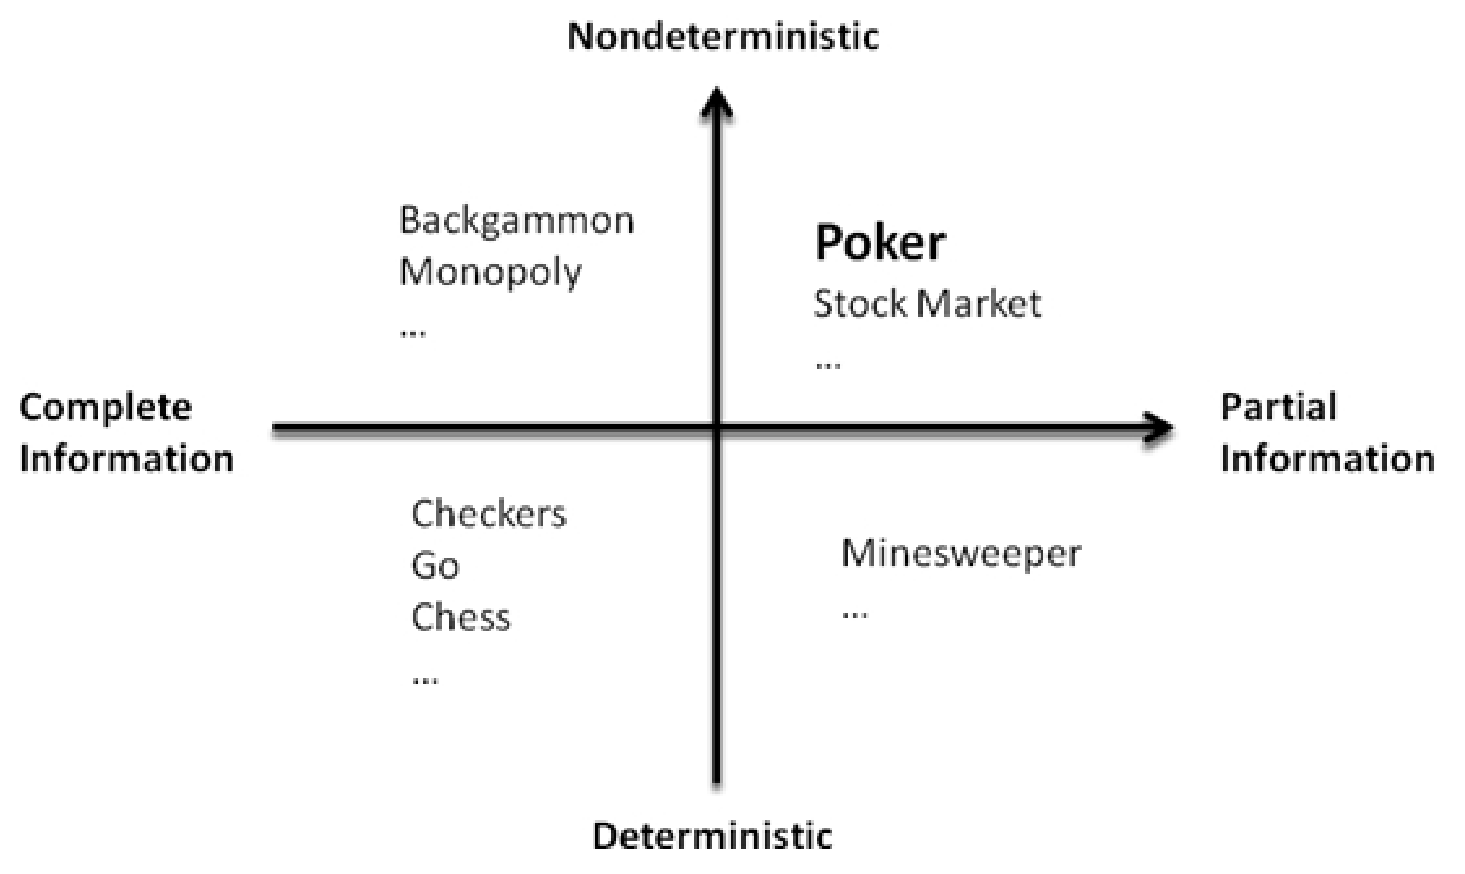
\includegraphics[width=0.5\textwidth]{./img/classification.pdf}
           \caption{Charakterystyka gier  \cite{poker}.}
\end{figure}

Dodatkowo ważnym elementem jest umiejętności obserwacji gry oraz wybór prawidłowej strategii. Na podstawie
tego, można sklasyfikować graczy na cztery kategorie. 

\subsubsection{Loose Passive}

Osoba, która bardzo często wchodzi do gry niezależnie czy karty, które posiada, dają jej
wysokie szanse na wygraną. Ten typ gry charakteryzuje się częstym wykonywanie akcji 'call' oraz
małą ilością przebić stawki \cite{class}. 

\subsubsection{Loose Aggressive}

Ten typ gry określa osobę, która często wykonuje akcję 'raise' i 're-raise' 
pod warunkiem, że ma silne karty \cite{class}. W innym przypadku wyrównuje żetony do aktualnej stawki.
Taka strategia okazuje się nieefektywna w przypadku gry z osobami, które często wchodzą do gry 
niezależnie od kart jak na przykład typ 'Loose-Passive' \cite{class}. 

\subsubsection{Tight Passive}

Można poznać tę kategorię gry przez to, że uczestnik wchodzi tylko z dobrymi kartami i często 
pasuje przy spotkaniu z graczem agresywnym, który przebija. Taki gracz traci wiele okazji, kiedy
mógłby wygrać \cite{class}. 

\subsubsection{Tight Aggressive}

Typ gry popularny wśród profesjonalnych graczy i najtrudniejszy do opanowania \cite{class}.




\begin{figure}[h!]
            \center
           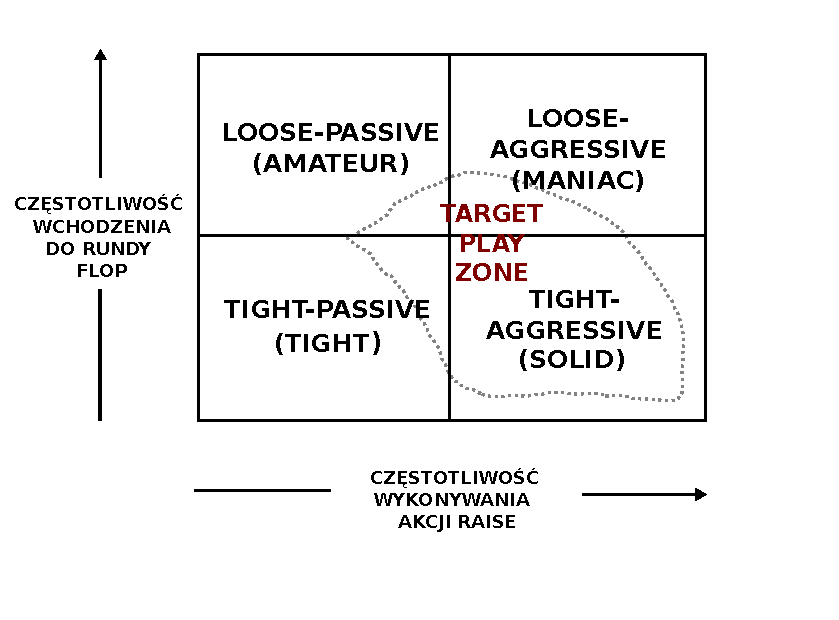
\includegraphics[width=0.5\textwidth]{./img/class.pdf}
           \caption{Podział graczy \cite{class}.}
\end{figure}


Jak wynika z powyższych kategorii, gra 'Poker Texas Hold'em' zawiera wiele elementów niezwiązanych z
losowością, gdzie obserwacje i dobieranie odpowiedniej strategi do typu gracza pełni kluczową
funkcję. W takim
wypadku jest uzasadnione wysunięcie tezy, że można utworzyć sztuczną inteligencję,
która będzie bazować na podobnych założeniach, które mogłyby być charakterystyczne
dla profesjonalnych graczy.

\section{Uczenie przez wzmacnianie}

Jest wiele sposobów na tworzenie sztucznej inteligencji do gier, między innymi można użyć technik uczenia
nadzorowanego pod warunkiem, jeśli przygotuje się odpowiednie zbiory danych. W pracy jednak
zdecydowano się na uczenie przez wzmacnianie. Wynika to z faktu, że jest mało publicznych zapisów
gry profesjonalnych graczy, które mogłyby posłużyć jako zbiory uczące.
Algorytmy należące do
wybranego działu uczenia powinny być w stanie polepszać swoje wyniki na podstawie interakcji ze
środowiskiem bez korzystania z zewnętrznych materiałów.  


Wiele istniejących algorytmów należących do wybranej techniki zakłada, że środowisko można opisać
przez model
matematyczny
MDP (\emph{Markov Decision Process}). 
Określa ona sekwencyjnie podejmowane decyzje w niepewnym środowisku \cite{mdp}. W każdym z nowych
stanów, w
jakich znajduje się \emph{Agent}, wykonuje on pojedyńczą akcję, zyskując od środowiska informacje o nowym stanie
oraz nagrodzie. Elementem wyjściowym zasady powinien być
zbiór strategii w postaci modelu, rys. 2.3.


\begin{figure}[th!]
            \center
           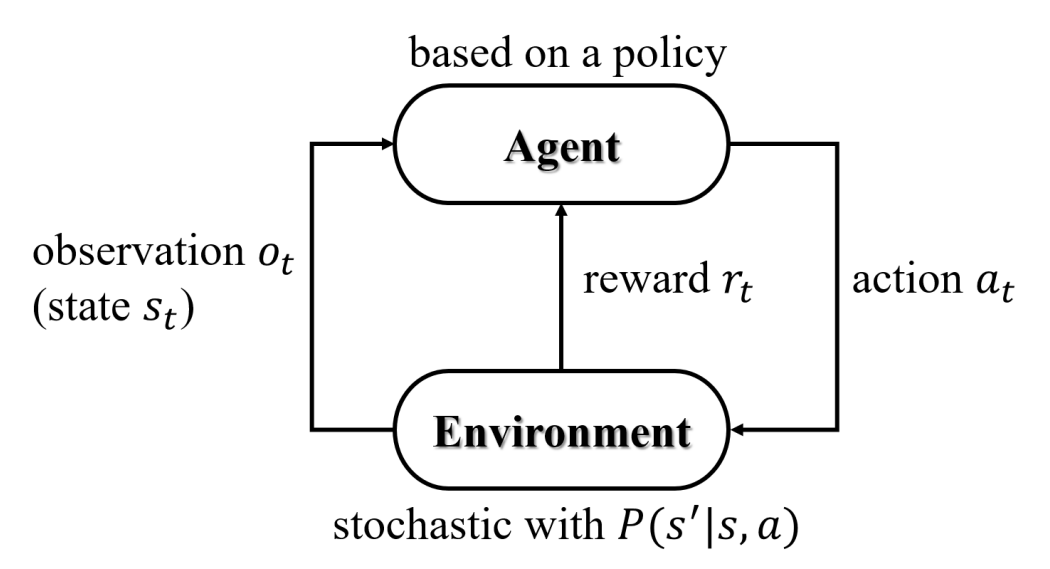
\includegraphics[width=0.5\textwidth]{./img/MDP.png}
           \caption{Schemat interakcji ze środowiskiem \cite{mdp}.}
\end{figure}


MDP może opisywać jedynie środowiska z pełnym zakresem informacji, w przypadku algorytmu będącego
tematem pracy, głównym zadaniem jest rozwiązanie środowiska z niepełnym zestawem danych. Wtedy 
należy rozpatrywać zasadę Partially Observable Markov Process, POMDP \cite{mdp}.


\vspace{2cm}
W przeciwieństwie do poprzedniej zasady tutaj agent nie zna aktualnego stanu, w którym
się znajduje \cite{mdp}. Przez takie okoliczności musi połączyć zależnością wykonywane akcie i
obserwacje, a nie stany. Większość gier karcianych można zakwalifikować do tego typu problemów
\cite{mdp}. Dodatkowo gry karciane można powiązać z terminem "Teoria Gier".

\section{Teoria Gier}

Aby zrozumieć działanie algorytmów CFR, Deep CFR, MCCFR itd. należy zapoznać się
z podstawami działu matematyki o nazwie Teoria Gier. Bada on optymalne zachowanie w środowiskach gdzie
występuję konflikt \cite{gt}. W przypadku gry Poker Texas
Hold'em zostaną wytłumaczone tylko takie terminy jak Równości Nasha lub
gra w postaci ekstensywnej.

\subsubsection{Gra w postaci ekstensywnej}

Gry w
formie ekstensywnej można przedstawić jako drzewo decyzyjne, gdzie każdy węzeł rozgałęzia się na
możliwe akcje oraz identyfikuje aktualny stan gracza przez zestaw informacji,
ostatnie węzły to stany końcowe gdzie określony gracz zyskuje nagrodę lub ją traci \cite{gt}.
Jest to sposób
na uproszczenie opisu gry.

Na rys. 1.4 przedstawiono przykład gry 'Papier-Kamień-Nożyce' w formie ekstensywnej, gdzie gracze P1 i
P2 eksplorują 3 akcie w swoich węzłach. 


\begin{figure}[th!]
            \center
           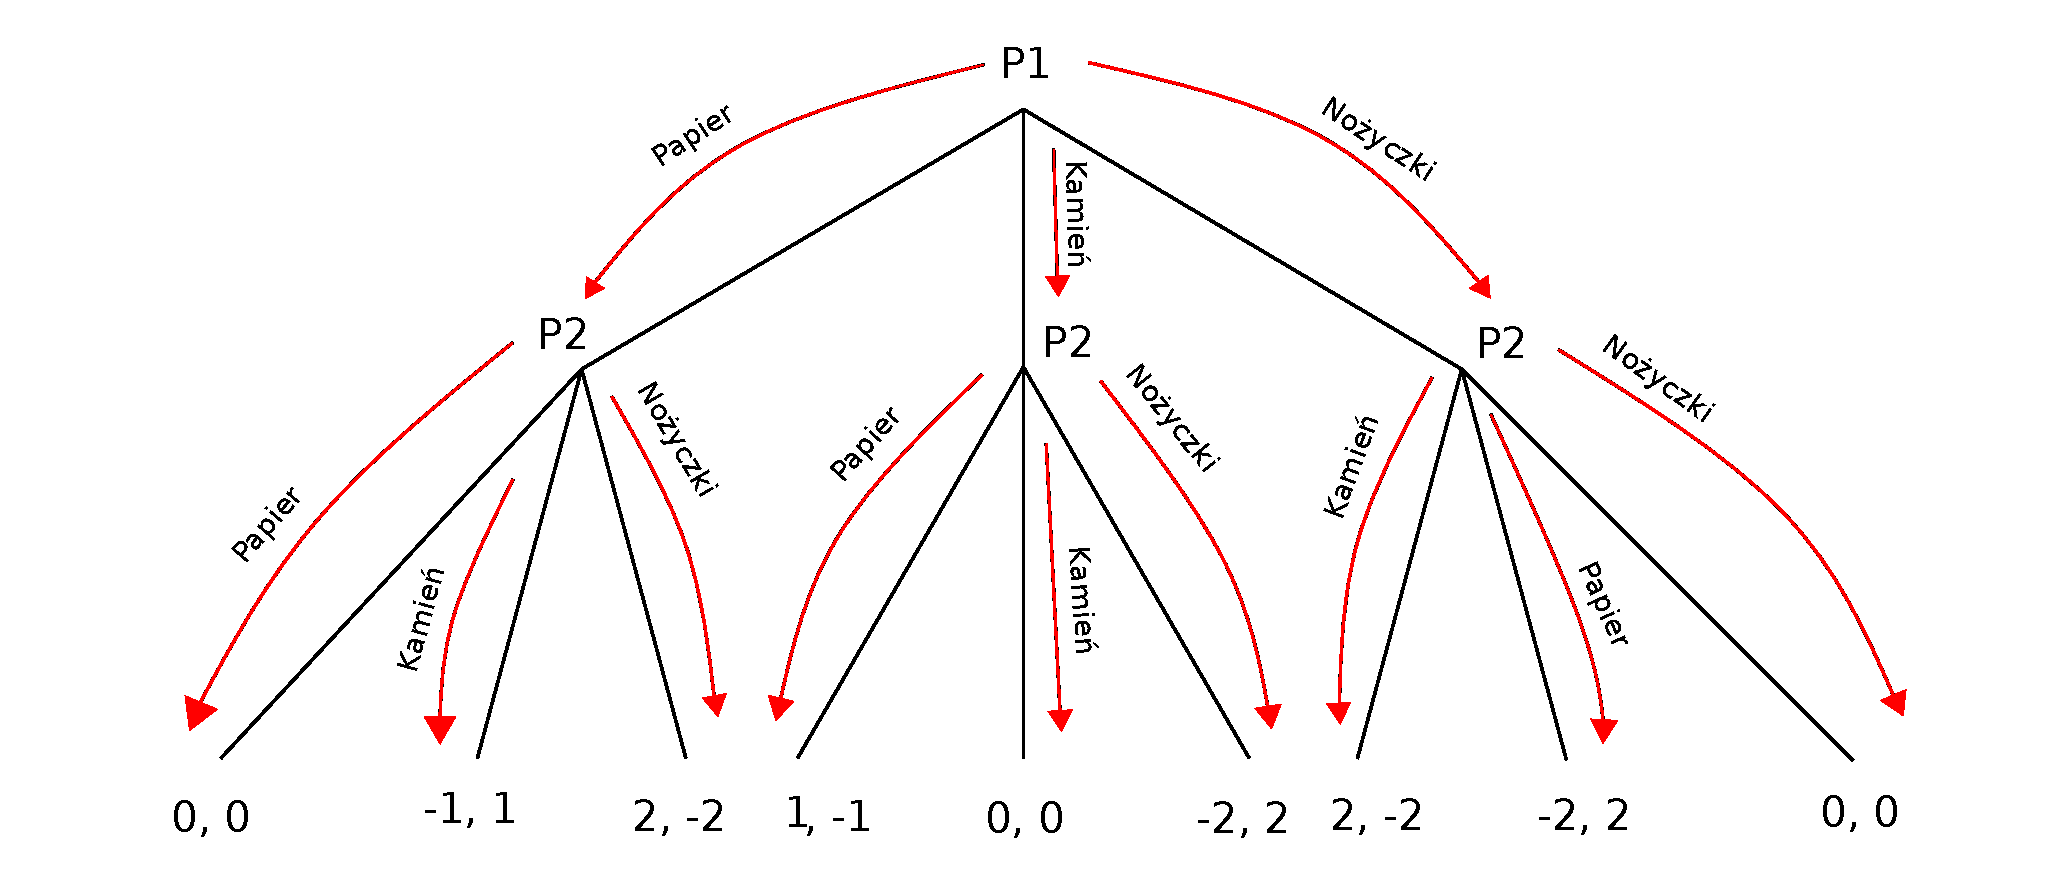
\includegraphics[width=0.9\textwidth]{./img/drawing1.pdf}
           \caption{przykład gry w postaci ekstensywnej.}
\end{figure}

Każdy z graczy eksploruje wyniki swoich akcji oraz zapamiętuje dotychczasową historię, co może zostać potem
wykorzystane do znalezienia najbardziej opłacalnych ścieżek.

\vspace{5cm}
\subsubsection{Równowaga Nasha}

W grach to twierdzenie określa perfekcyjny stan gry, gdzie wszyscy gracze wykorzystują najlepszy
zestaw strategii, którego zmiana przyniesie tylko straty. Oznacza to, że nie jest możliwa
zmiana ruchów oraz zwiększenie uzyskanej nagrody \cite{gt}. 

Dobrym przykładem prezentującym taki stan jest "Dylemat Więźnia" \cite{rn}. To środowisko zawiera 
dwóch przestępców, którzy są przesłuchiwani w odseparowanych pomieszczeniach. Każdy z nich ma dwie
opcje, przyznać się do zarzutów lub tego nie robić. Każda z kombinacji akcji uczestników jest
zaprezentowana w tab. 2.1, gdzie wartości określają lata spędzone w więzieniu po danym ruchu.


Posługując się Równowagą Nasha, można stwierdzić, że najlepszą opcją dla
obu uczestników będzie przyznawanie się za każdym razem \cite{rn}. Wynika to z faktu, że wyniki
przegranej są tam małe wraz z brakiem ryzykowania porażką, czyli 5 latami w więzienia.

\vspace{1cm}
\begin{table}[h!]
   \centering
\caption{Wyniki akcji środowiska "Dylemat więźnia".}
\begin{tabular}{|c|c|c|}
   \hline
   & \makecell{przyznanie się \\ więźnia A} & \makecell{więzień A \\ kłamie} \\ 
   \hline
   \makecell{przyznanie się \\ więźnia B} & \diagbox[innerwidth=3cm]{1}{1} & \diagbox[innerwidth=3cm]{0.5}{5} \\
   \hline
   \makecell{więzień B \\ kłamie} & \diagbox[innerwidth=3cm]{5}{0.5} & \diagbox[innerwidth=3cm]{0}{0} \\
   \hline
\end{tabular}

\end{table}



\section{Historia modeli Texas Hold'em Poker}

Bazując na teorii gier oraz różnych algorytmach powstało wiele rozwiązań różnych wersji gry Poker.
Pierwsze dokumenty naukowe omawiały bardzo proste
środowiska jak Poker Kuhn.
Dopiero w 2015 roku utworzono pierwszą znaną sztuczną inteligencję $"\text{Cepheus}"$ rozwiązującą problem
HULH przez algorytm CFR+ \cite{cepheus}. Po tym osiągnięciu rozpoczęto prace nad
algorytmem mogącym rozwiązać problem gry HUNH (\emph{Heads Up No-limit Texas Hold'em}).
Powstały model nazwano "DeepStack". Mieszał on sieci neuronowe z 
technikami algorytmu CFR. 
Przetestowano go na 33 profesjonalnych graczach w wielu iteracjach gry. Algorytm w większości
przypadków wygrał \cite{ds}. Była to pierwsza wygrana AI z człowiekiem w normalnej 
wersji gry Poker Texas Hold'em. 

Jak pokazują dotychczasowe osiągnięcia Poker Texas Hold'em jest bardzo skomplikowanym środowiskiem 
do uczenia maszynowego. Sposoby na jego rozwiązanie zaczęły powstawać od niedawna, a pierwsze
duże osiągnięcie w grze HUNH miało miejsce dopiero w 2017 roku. 

\section{Counterfactual Regret Minimization}

\subsection{Regret Matching}

Jest to nieodłączna metoda uczenia AI w grach karcianych. Polega ona na liczeniu najlepszej 
strategii pod warunkiem, że znany jest wektor żalu w węźle.
Taki wektor opisuje się jako tablicę wag o długości równej liczbie możliwych akcji gracza. Każda z 
tych wag opisuje stopień opłacalności danego ruchu.


Poniżej przedstawiono wzór wynikający z tej metody, gdzie  
$R^{t}(I, a)$ jest omawianym wektor \cite{CFR}. 
Następnie aby uzyskać nową strategię, usuwa się wartości ujemne (formuła nr 1.2) 
i sprawdza, czy ich suma jest 
większa od zera. W zależności od tego warunku wybierany jest rozkład, wzór nr 1.1.


\begin{equation}
p^{t}_{i}\left( a \right) = \left\{ \begin{array}{ll}
      \frac{R^{T, \text{+}}\left(a\right)}{ \Sigma_{a' \in A} R^{T,\text{+}}\left(a'\right)} &
      \mbox{if $\Sigma_{a' \in A} R^{T,\text{+}}\left(a'\right) >
      0$};\\
      \frac{1}{|A|} & \mbox{$otherwise$}.\end{array} \right. \ 
\end{equation}

\vspace{1cm}
\begin{equation}
   R^{t,\text{+}}(a) = max(R^t(a),0)
\end{equation}


Proces ten jest powtarzany wielokrotnie, tak, aby przy każdej iteracji rozkłady prawdopodobieństwa
ruchów były stopniowo
poprawiane.

W przypadku algorytmu Deep CFR, zachodzi modyfikacja formuły nr 1.1. Strategia jest liczona na
dodatnich wartościach żalu podzielonego przez  prawdopodobieństwo dostania się do 
tego stanu $D^{T} (I, a)$ \cite{DCFR}.
Jeśli suma jest ujemna to zostaje wybrana akcja z najwyższą wartością $D^{T}(I, a)$ \cite{DCFR}.



\begin{equation}
\sigma^{t+1}_{i}\left(I, a \right) = \left\{ \begin{array}{ll}
      \frac{D^{T, \text{+}}\left(a\right)}{ \Sigma_{a' \in A} D^{T,\text{+}}\left(a'\right)} &
      \mbox{if $\Sigma_{a' \in A} D^{T,\text{+}}\left(a'\right) >
      0$};\\
      \text{argmax}(D^{T} (I, a)) & \mbox{$otherwise$}.\end{array} \right. \ 
\end{equation}



\subsection{Counterfactual Regret}

Algorytm CFR do znanych wcześniej metod dodał termin 'Immediate Counterfactual Regret' oznaczany przez $R^{T}_{i,
imm} (I)$, 
czyli żal przydzielony do węzła I.
Do obliczenia takiego parametru została zdefiniowana wartość "counterfactual utility" $u_{i}(\sigma,
I)$. Oznacza ona przewidywany wynik nagrody dla stanu I gdzie wszyscy gracze używają strategi
$\sigma$, \cite{CFR}. Dodatkowo $\pi^{\sigma} (h, h')$ oznacza prawdopodobieństwo dostania się z historii h do 
nowego stanu h' przy strategii $\sigma$ \cite{CFR}.

\begin{equation}
   u_{i} (\sigma, I) = \frac{\sum_{h \in I, h' \in Z} \pi^{\sigma}_{-i} (h) \pi^{\sigma} (h,
   h') u_{i}(h')}{\pi_{-i}^{\sigma}(I)}
\end{equation}

Na podstawie równania 2.5 można wyliczyć końcową wartość żalu w algorytmie CFR.

\begin{equation}
   R^{T}_{i,\text{imm}} (I, a) = \frac{1}{T} \sum^{T}_{t=1} \pi^{\sigma^{t}}_{-i} (I)
   (u_{i}(\sigma^{t}|_{I \rightarrow a}, I) - u_{i}(\sigma^{t}, I))
\end{equation}


Powyższe 2 równania można doprowadzic do formuły nr 2.6. Wartość $\pi^{\sigma} (h,h')$ została
zastąpiona przez 1, ponieważ
CFR zakłada, że dla $u_{i}(\sigma^{t}|_{I \rightarrow a}, I)$, gracz wykonuje zawsze akcję \emph{a} \cite{CFR}.



\begin{equation}
   R^{T}_{i,\text{imm}} (I, a) = \frac{1}{T} \sum^{T}_{t=1}
   \pi_{-i}^{\sigma}(h)\sum_{h \in I, h' \in Z}(1*u_{i}(h') - \pi^{\sigma}(h,h')u_{i}(h'))
\end{equation}


\vspace{0.5cm}
Po uzyskaniu $R^{T}_{i,\text{imm}} (I, a)$ można wykorzystać metodę "Regret Matchning" i
zaktualizować strategie.
Poniżej przedstawiono przykład obliczeń pojedyńczego węzła oraz wyniki 
dla gry 'Papier-Kamień-Nożyce' przy ustawionych
nagrodach i karach w stanach końcowych jak na rys. 2.5, 2.6, 2.7.

\begin{center}
$$
   \pi^{\sigma}(h,h')u_{i}(h') =  (\frac{1}{3} \cdot 0) + (\frac{1}{3} \cdot -1) +
   (\frac{1}{3} \cdot 2) = \frac{1}{3}
$$

$$
T*R^{T}_{i,\text{imm}} (I, a) =
((0-\frac{1}{3}), (-1-\frac{1}{3}), (2-\frac{1}{3})) \cdot \frac{1}{3}= (-\frac{1}{9},
-\frac{4}{9}, \frac{5}{9}) 
$$

$$
\sigma^{t+1}_{i}\left(I, a \right) = (0, 0, 1)
$$
\end{center}
\vspace{0.5cm}


\begin{figure}[th!]
            \center
           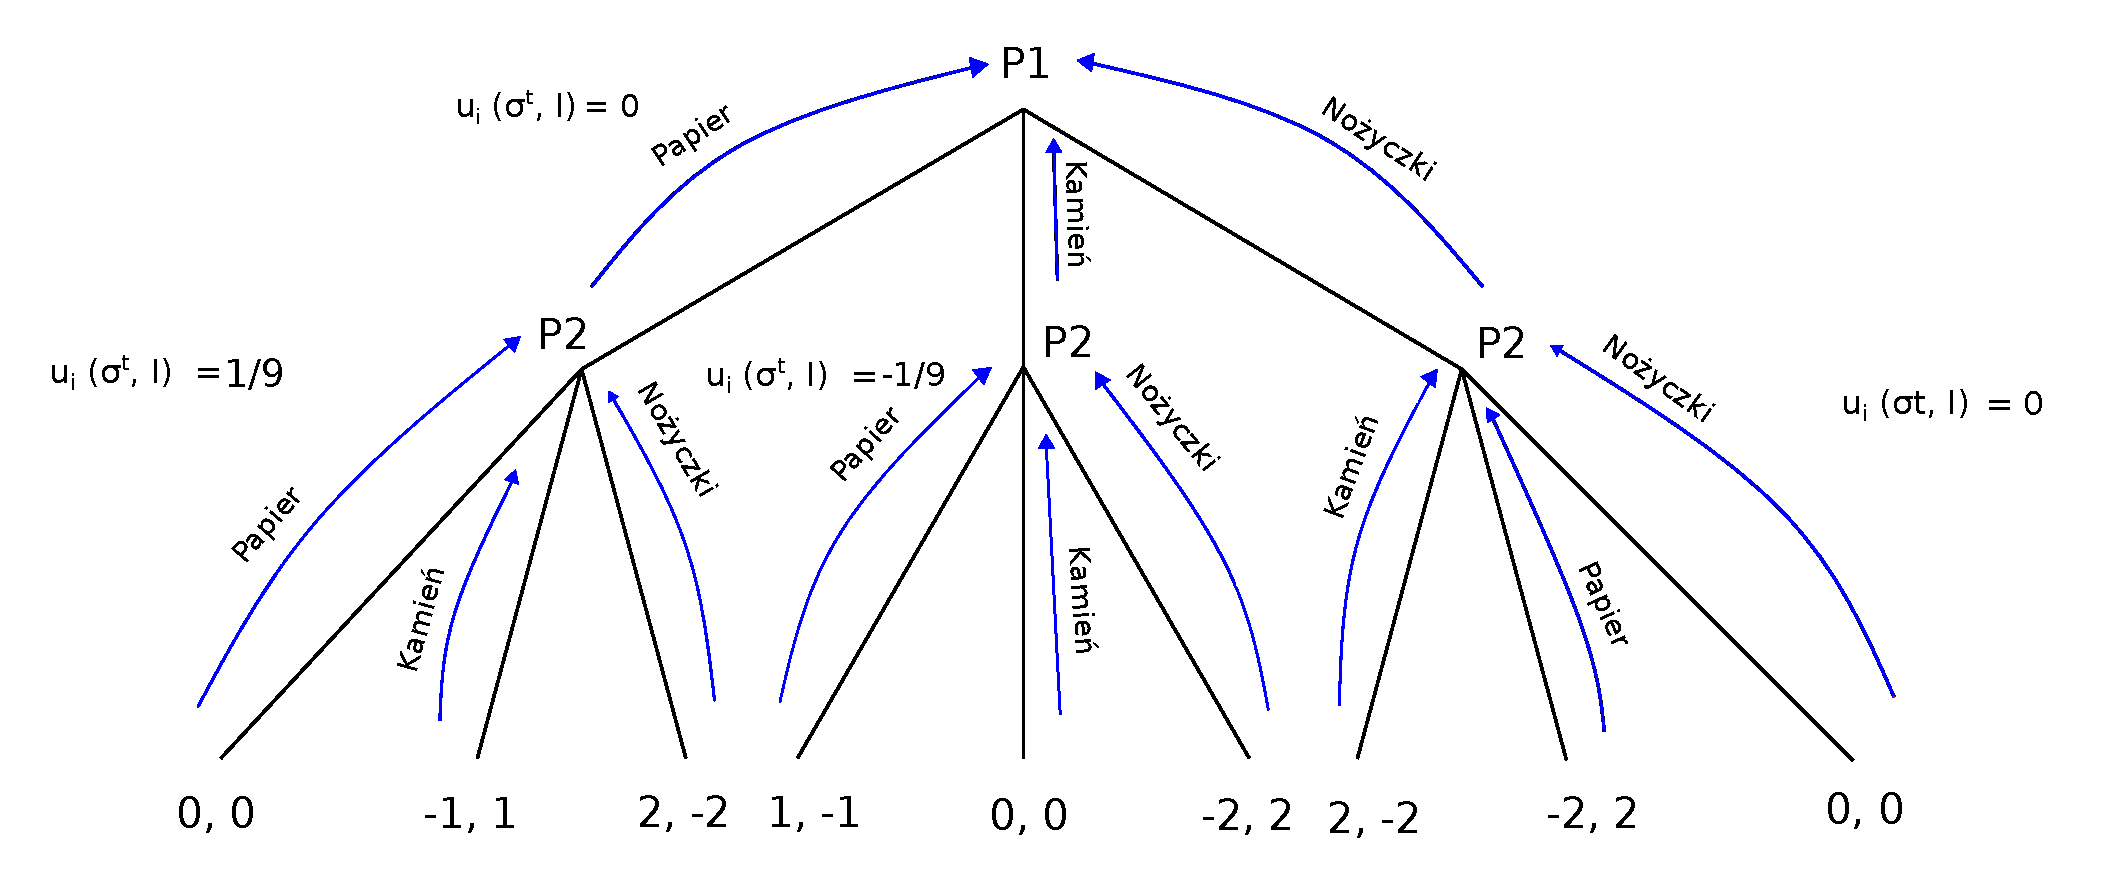
\includegraphics[width=1\textwidth]{./img/drawing2.pdf}
           \caption{Przykład 'counterfactual utility'.}
\end{figure}

Na podstawie rys. 2.5 widać, że gracz P2 będzie miał stan o najwyższej wartości "counterfactual utility" w węźle $u_{i}
(\sigma^{t}, I)=\frac{1}{9}$, a najniższej dla $u_{i}(\sigma^{t}, I)=-\frac{1}{9}$.


\begin{figure}[th!]
            \center
           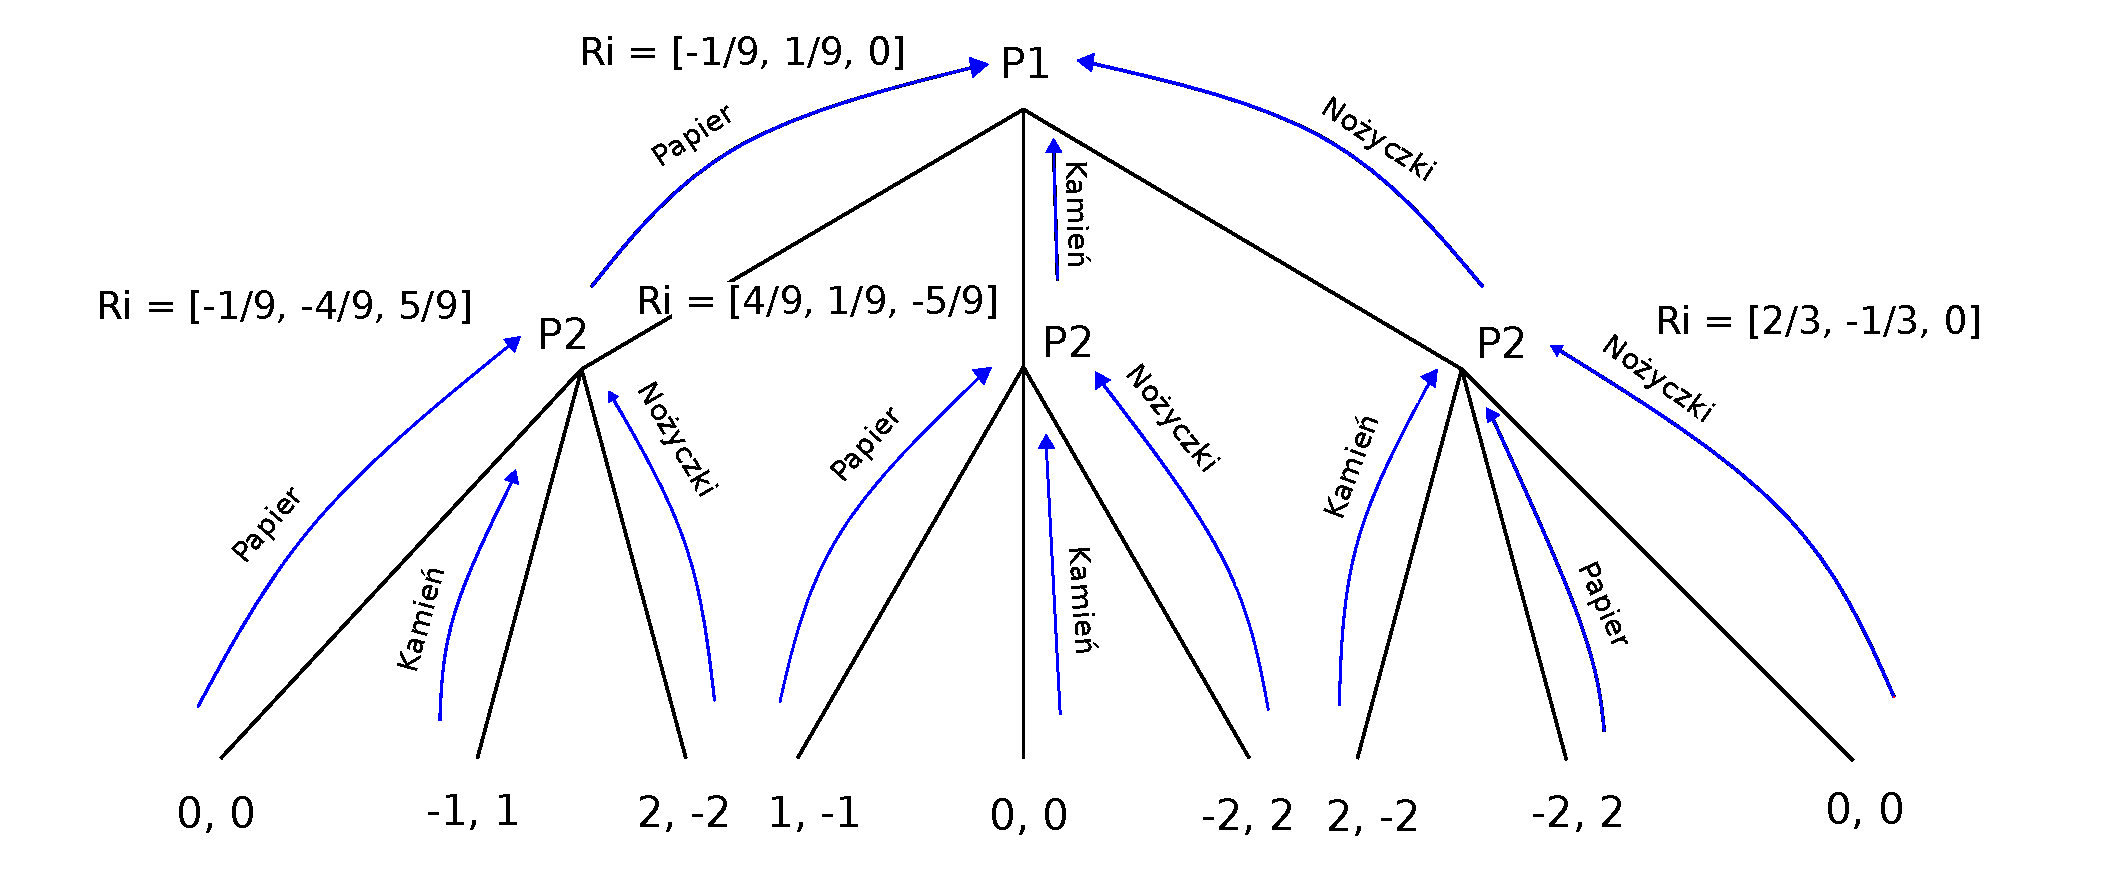
\includegraphics[width=1\textwidth]{./img/drawing3.pdf}
           \caption{Przykład 'Immediate Counterfactual Regret'.}
\end{figure}

\vspace{0.5cm}
\vspace{10cm}

Powyżej zaprezentowano wektory $R^{T}_{i,\text{imm}} (I, a)$.
Gracz P1 grając, najbardziej będze żałował nie wykonania akcji 'Kamień', a najmniej 'Papier'.

\vspace{0.5cm}
\begin{figure}[th!]
            \center
           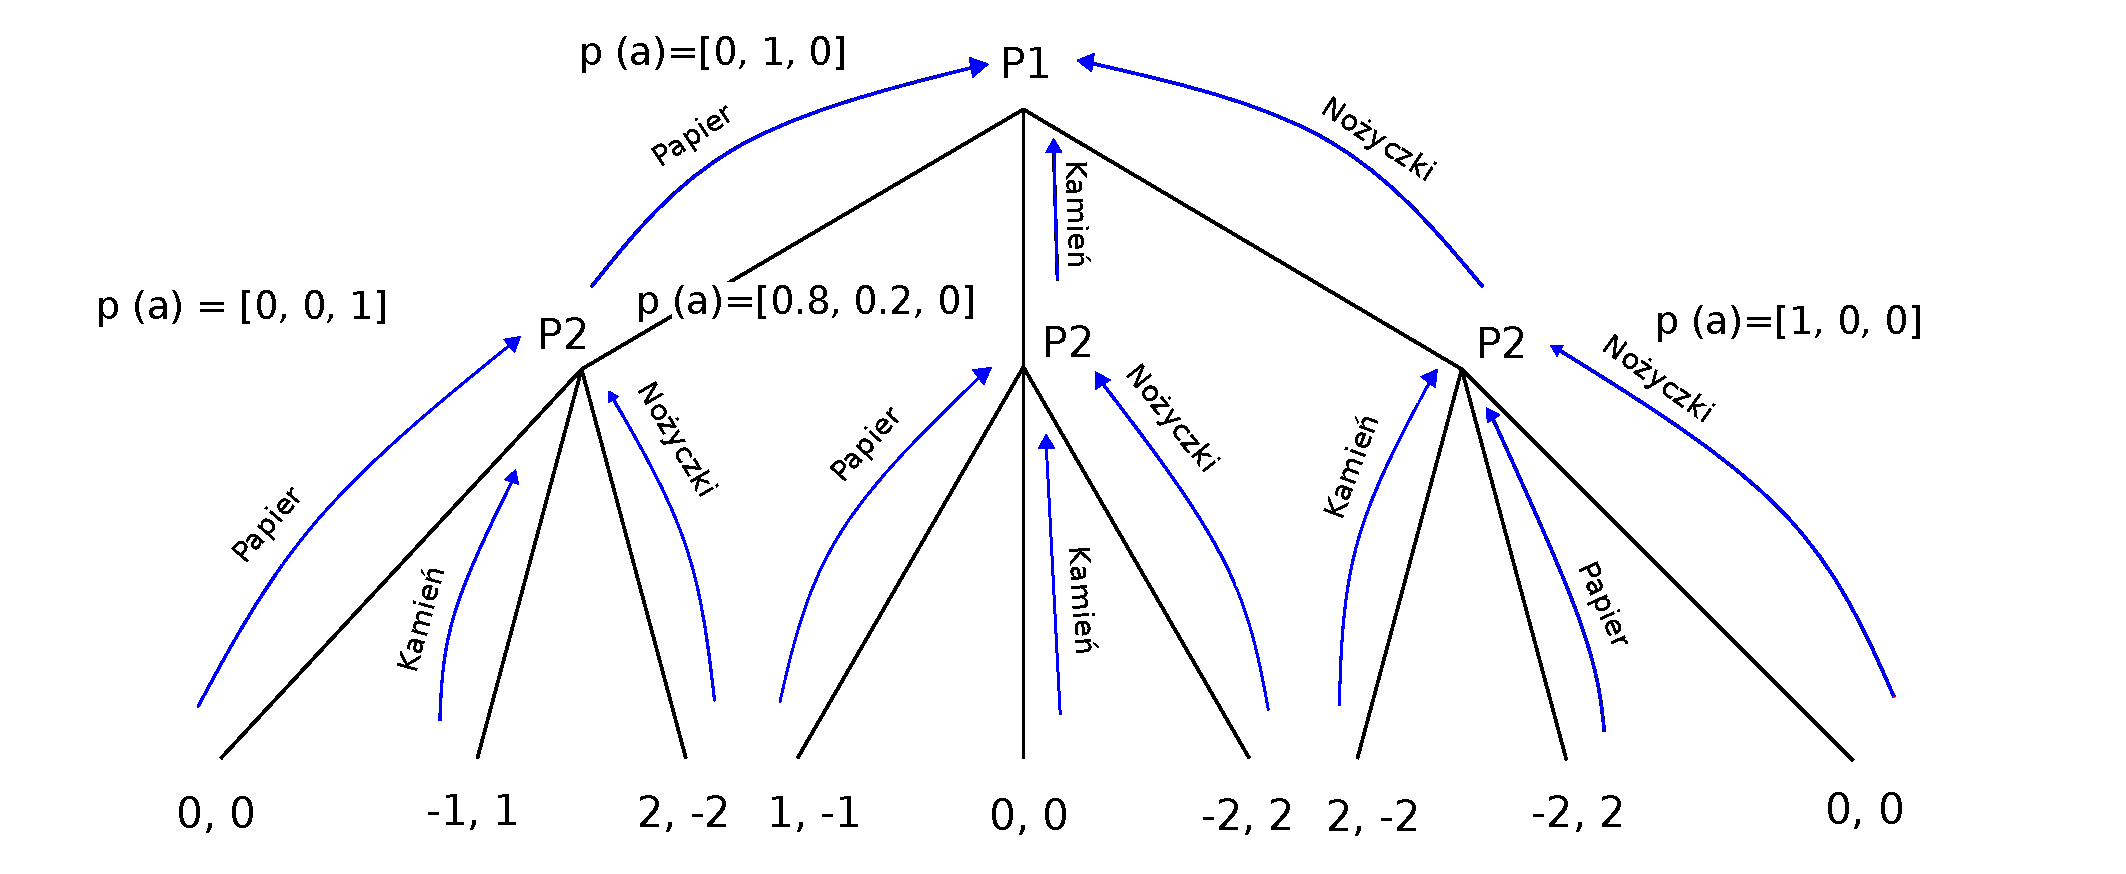
\includegraphics[width=1\textwidth]{./img/drawing4.pdf}
           \caption{Przykład strategii.}
\end{figure}
 
Rys. 2.7 przedstawia wektory określające jakimi rozkładami akcji powinni się kierować gracze, aby
osiągnąć najlepsze wyniki. Są to wektory wyliczone po pierwszej iteracji, w praktyce eksploracja
drzewa i powyższe obliczenia są powtarzane wielokrotnie. Końcowym etapem algorytmu CFR jest
policzenie średniej strategii \cite{CFR}.





\subsection{Monte Carlo Conterfactual Regret Minimization}

Algorytm CFR eksploruje całe drzewa decyzyjnego w jednej iteracji, co tworzy wymagania na
dużą moc obliczeniową i długi czas uczenia. Dla małych gier takie rozwiązanie jest akceptowalne, ale w przypadku 
większych środowisk jest nieefektywny.
Spowodowało to powstanie nowszej wersji algorytmu, MCCFR ('\emph{Monte Carlo Conterfactual Regret
Minimization}') , 
który w każdą iterację eksploruje tylko część drzewa \cite{mccfr}.

Metodę można podzielić na dwie odmiany, Outcome-Sampling oraz External-Sampling \cite{mccfr}.

W pracy zostanie przedstawiony sposób MCCFR ES ('\emph{Monte Carlo Conterfactual Regret
Minimization External Sampling}'), ponieważ taki został zaimplementowany w algorytmie
Deep CFR.
MCCFR ES przed eksploracją drzewa wybiera kolejno spośród graczy jednego uczestnika, którego 
oznacza
się jako 'traverser'.
Eksploruje on wszystkie odpowiedzi ze swoich akcji w danym węźle. W międzyczasie inni
uczestnicy wykonują pojedynczy ruch na podstawie wybranej strategii \cite{mccfr}.  


Na rys. 2.8 przedstawiono przykład część drzewa HULH, 
gdzie gracz 'P2'
został wybrany jako 'traverser'. 
Jak można zauważyć, tylko jego węzły rozgałęziają się na wszystkie możliwe ścieżki. 
Dodatkowo w drodze powrotnej obliczono $u_{i} (\sigma, I)$ dla wszystkich
stanów używając wzoru 
1.5.


\begin{figure}[!ht]
  \centering
  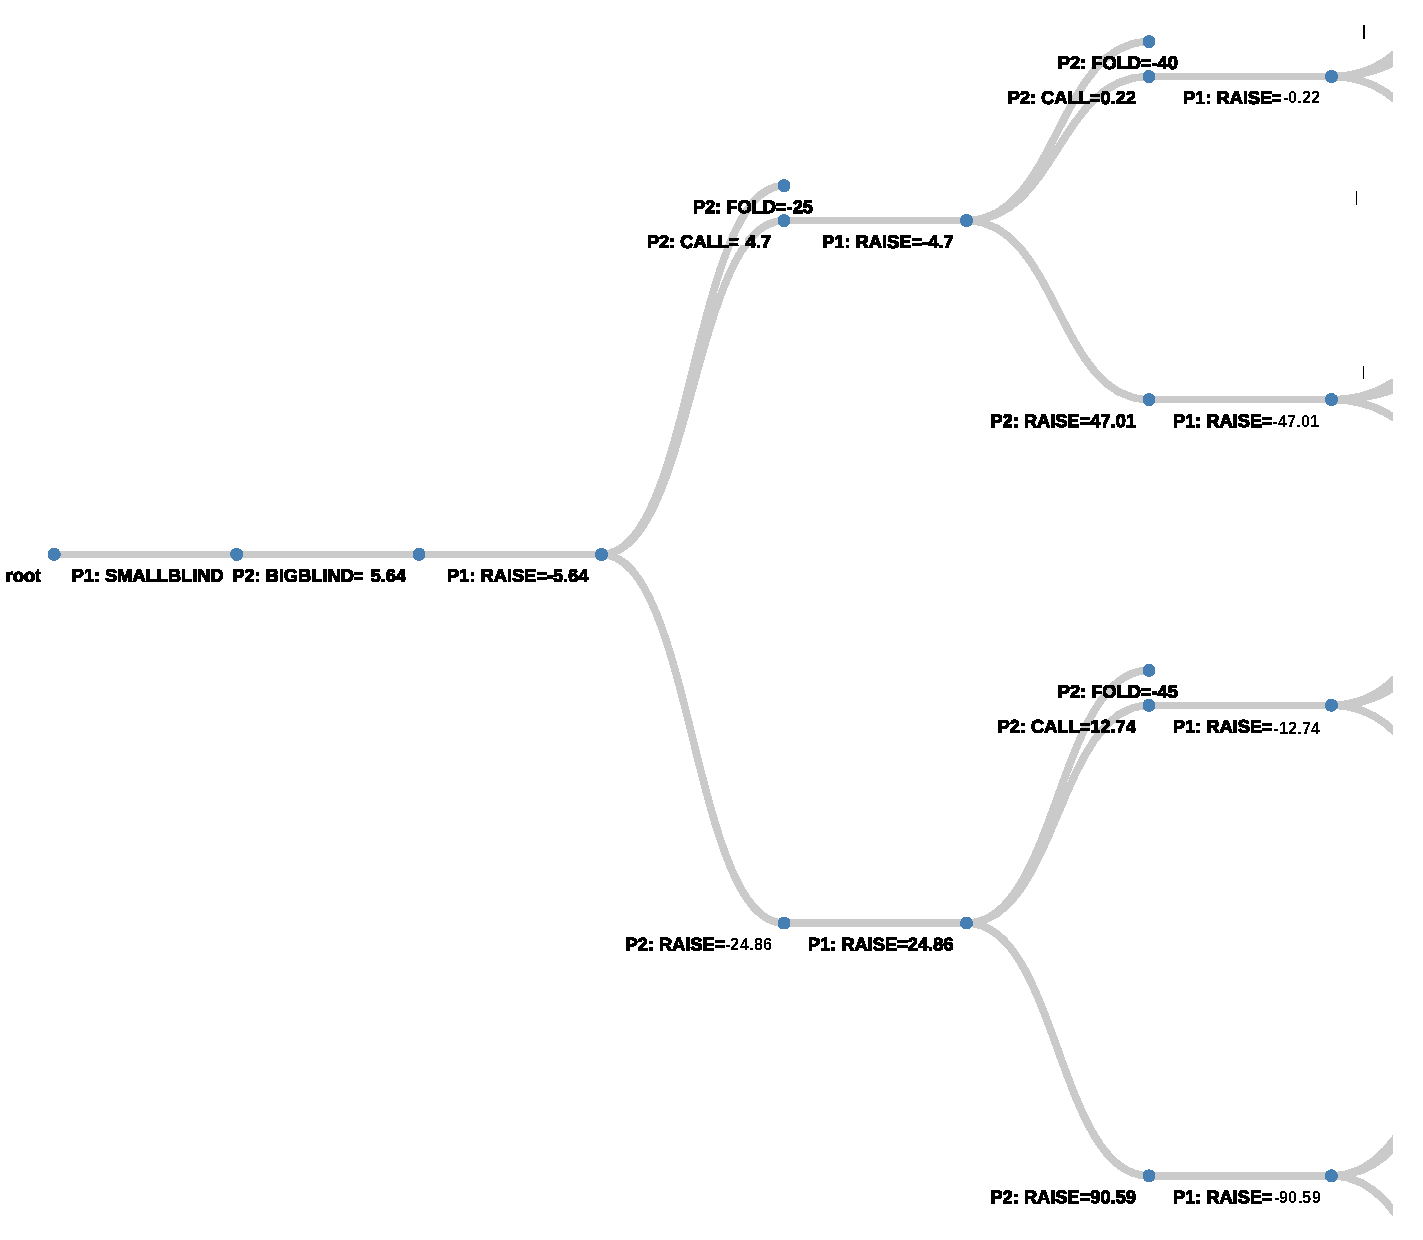
\includegraphics[width=1\textwidth]{./img/tree.pdf}
  \caption{Część drzewa decyzyjnego MCCFR ES z graczem P2 jako traverser.}
\end{figure}


\vspace{5cm}
Jest to przykład z jednej eksploracji gry, w praktyce powtarza się ten proces wielokrotnie, 
uzyskując różne wersje gry.


Mając takie drzewo, można przystąpić do liczenia $R_{i,imm}^{T} (I)$ oraz poprawiania 
wyników przez Regret Matching. MCCFR ES spełnia swoją funkcję, ale wymaga wielu iteracji, aby
uzyskać dobre wyniki. Z tego powodu w dalszym rozdziale zostanie przedstawiona metoda Deep CFR,
która przyspiesza proces uczenia przez użycie sieci neuronowych.

\section{Deep CFR}


Algorytm Deep CFR rozwija podstawową wersję metody CFR o sieci neuronowe.
Taka modyfikacja była wymagana, aby utworzyć algorytm, który może rozwiązać nie tylko proste gry,
ale też i duże jak HULH. Liczy on wektory w drzewie decyzyjnym
przez algorytm MCCFR ES. Dodatkowo Deep CFR zbiega się do Równości Nasha szybciej niż 
popularny algorytm NFSP z 2016 roku \cite{DCFR}.

Deep CFR wykorzystuje sieci neuronowe do przewidzenia wartości $D^{T}$(I, a) w podobnych
obserwacjach, potem na
podstawie predykcji liczy strategię ze wzoru nr 1.3.   
Następnie liczona jest zaktualizowana wersja wektora żalu, formuła nr 1.5.
Obliczone wyniki są dodawane do buforów $B_{1}$, $B_{2}$, a strategia do zbioru $B_{s}$.


Po wielu iteracjach
rozpoczyna się nauka sieci z zebranej bazy. Poniżej przedstawiono dokładny opis Deep CFR.
\vspace{1cm}

\begin{algorithm}[H]
\SetKwInput{KwInput}{Wejście}                % Set the Input
\SetKwInput{KwOutput}{Wyjście}              % set the Output
\DontPrintSemicolon
  
\KwInput{$B_{p}$, $B_{s}$, $\theta_{s}$, $\theta_{p}$, $P$, $N$, $K$}
\KwOutput{$\theta_{s}$}
\For{n \textbf{in} $N$}{
   $h$, $t$ \leftarrow \text{Nowa gra}\\
   \For{$p$ \textbf{in} $P$}{
      \For{$k$ \textbf{in} $K$}{
         MCCFRES($\theta_{p}$, $\theta_{p-1}$, $p$, $t$, $h$, $B_{p}$, $B_{s}$)\\
      }
      $\theta_{p}$ \leftarrow \text{TRAIN($B_{p}$, $\theta_{p}$, $t$)} \Comment{loss:
         $\frac{1}{N_{batch}}$
      $\sum(y_{i}-\widehat{y_{i}})^2$$\cdot$$t_{i}$}\\
   }
}
$\theta_{s}$ \leftarrow \text{TRAIN($B_{s}$, $\theta_{s}$, $t$)} \Comment{loss:  $\frac{1}{N_{batch}}$$\sum(y_{i} -\widehat{y_{i}})^2$$\cdot$t_{i}$}\\
\textbf{return} $\theta_{s}$
 \caption{Deep CFR}
\end{algorithm}

\vspace{1cm}
Algorytm na wejściu dostaje argumenty przystosowane do gry 2-osobowej.
Pierwszymi elementami są bufory graczy $B_{p}$ ($B_{1}$, $B_{2}$) oraz kontener na 
strategie $B_{s}$.
Dodatkowo metoda potrzebuje listę uczestników P, z których będzie wybierać 'traversera'.
Ostatnimi argumentami są iteracje gry N oraz liczba eksploracji drzewa K.


W metodzie należy ustawić trzy pętle wraz z nową rundą uzyskując początkową historię oraz
krok gry t. Kolejnym etapem jest
wykonanie funkcji \emph{MCCFRES}. Przyjmuje ona na wejściu sieci neuronowe obu graczy, 
listę uczestników p,
numer kroku t, historię rundy h oraz bufory. Po k 
powtórzeniach następuje uczenie sieci neuronowej wybranego wcześniej gracza jako 'traversera'. 

Model używa 
zmodyfikowanej wersji funckcji MSE do liczenia błędu predykcji. Każdy wynik $(y_{i} - \hat{y_{i}})^2$
mnożony jest przez krok $t_{i}$ w, którym uzyskano $y_{i}$ \cite{DCFR}.
Dodatkowo jak wynika z badań algorytm osiąga lepsze wyniki
jeśli
sieci neuronowe są trenowane od początku \cite{DCFR}. Dlatego należy przed funkcją \emph{TRAIN}
wyczyścić model.

Po wszystkich powtórzeniach i zebraniu całej bazy bufora $B_{s}$ rozpoczyna się trenowanie sieci 
neuronowej $\theta_{s}$ w ten sam sposób jak inne modele. Elementem wyjściowym Deep CFR jest 
$\theta_{s}$.


\vspace{1cm}
\begin{algorithm}[H]
\SetKwInput{KwInput}{Wejście}                % Set the Input
\DontPrintSemicolon
\SetKwFunction{FMain}{MCCFRES}
\SetKwProg{Fn}{Function}{:}{}
  
\Fn{\FMain{$\theta_{p}$, $\theta_{p-1}$, $p$, $t$, $h$, $B_{p}$, $B_{s}$}}{
   $t_{r}$ \leftarrow h \Comment{sprawdzenie czyja jest aktualnie tura}\\

   \uIf{$h$ jest stanem końcowym Z}{
      \textbf{return} $u_{p} (h)$
   }
   \uElseIf{$p$ = $t_{r}$}{
      $\hat{D}(I)$ \leftarrow \text{obliczenie wektora $\hat{D}(I)$ używając h}\\
      $\sigma (I)$ \leftarrow \text{Obliczenie strategi $\sigma_{t_{r}} (I)$, kożystając z $\hat{D}(I)$ i
         wzoru 1.1}\\

      \For{a \textbf{in} A(h)}{
         $u_{t_{r}}$(h) \leftarrow \FMain{$\theta_{p}$, $\theta_{p-1}$, $p$, $t+1$, $h+a$, $B_{p}$,$B_{s}$}\\
          
      }
      $u_{r_{r}}(\sigma, I)$ \leftarrow $\sum (u_{t_{r}}(h) \cdot \sigma(I))$\\
      $R^{T}_{t_{r}, imm}$(I) \leftarrow ($u_{t_{r}}(h) - u_{t_{r}}(\sigma, I)$)\\
      $B_{t_{r}}$ \leftarrow \text{dodanie próbki do bufora } $[R^{T}_{t_{r}, imm}$(I), h, t]$\\

   }
   \Else{
      $\hat{D}(I)$ \leftarrow \text{obliczenie wektora $\hat{D}(I)$ używając $\theta_{p}$ i
      stanu h}\\
      $\sigma (I)$ \leftarrow \text{Obliczenie strategi $\sigma_{p} (I)$, kożystając z $\hat{D}(I)$ i
         wzoru 1.1}\\
      $B_{s}$ \leftarrow \text{dodanie próbki do bufora } $[\sigma (I), h, t]$\\
      a \leftarrow $\sigma (I)$

      \textbf{return} \FMain{$\theta_{p}$, $\theta_{p-1}$, $p$, $t+1$, $h+a$, $B_{p}$,
         $B_{s}$}\\
   }
}
 \caption{Implementacja MCCFRES kożystając z sieci neuronowych}
\end{algorithm}

\vspace{1cm}

Implementacja MCCFR ES przedstawiona powyżej przy zadanych argumentach rozpoczyna się od
sprawdzenia, który gracz rozpoczyna daną turę. Na podstawie tej informacji będzie wykonywana
dalsza część algorytmu.


Pierwszym krokiem jest sprawdzenie, czy stan gry jest końcem gry. W przypadku prawdziwego 
warunku zwracana jest wygrana lub przegraną wartość stawki. 
Jeśli powyższy etap jest fałszywy, algorytm sprawdza, czy gracz jest oznaczony jako 'traverser'.
Wtedy program używając sieci neuronowej gracza,
otrzymuje wektor $\hat{D}(I)$ przez wprowadzenie do modelu informacji o widocznych kartach oraz
dotychczasowej historii gry. Korzystając ze wzoru 1.3, liczy strategie, odczytuje $u_{t_{r}}$ (h) 
wykonując rekurencję. Ostatnim krokiem jest wyliczenie wektora żalu i dodanie go do bufora.

Jeśli powyższy warunek był fałszywy, gracz liczy tak samo jak wcześniej $\hat{D}(I)$, nowy rozkład
akcji i dodaje ją do zbioru strategii. Następnie korzystając z tej sieci neuronowej i otrzymanej 
dystrybucji wykonuje nową akcję.


\section{Podsumowanie}

Środowiska z niepełnym zestawem informacji i brakiem deterministyczności są trudne do rozwiązania.
Algorytmy tworzące modele
dla takich gier są często skomplikowane i obciążające obliczeniowo. 
Przez takie cechy dopiero od niedawna zaczęły powstają algorytmy zdolne pokonać ludzi w 
dużych grach karcianych jak 'Cepheus' lub 'DeepStack'. 
Metody zdolne tworzyć takie AI dalej są rozwijane i aktualizowane z roku na rok.
W taki sposób w 2014 roku powstał CFR i MCCFR, po para latch zastąpiono je przez CFR+, a 
następnie
Deep CFR bedący tematyką pracy. 

Rozdział dokładnie opisał działanie omawianego algorytmu
przez przedstawienie terminów należących do działu matematyki 'Teoria Gier'. Między innymi
 pokazał, że opis środowiska przez drzewa decyzyjnych pozwala na wiele uproszczeń i możliwości
 śledzenia gry. Dodatkowo przedstawiono problem poszukiwania stanu Równości Nasha, którego
 znalezienie jest celem większości algorytmów sztucznej inteligencji gier karcianych.

Dobrzez zaimplementowany algorytm Deep CFR przy prawdidlowej parametryzacji i odpowiednio dużej
ilości iteracji powinien zbiec się do pókktu bliskiego takiego stanu.

\chapter{Implementacja algorytmu} 

Program Deep CFR został napisany w niniejszej pracy, korzystając z narzędzi
pozwalających na zredukowanie nadmiarowości kodu oraz na prostą implementację.
W tym rozdziale skupiono się na opisaniu wybranych technologii, parametrów oraz funkcji, 
które znalazły się w implementacji algorytm.

Bazą do napisanego kodu jest język programowania, Python 3.8. Zawiera on wiele
technologii wspomagających uczenie maszynowe i rozległą społeczność wspierającą jego rozwój.
Poniżej 
wy listowano i opisano główne narzędzia użyte w pracy.

\paragraph{TensorFlow}

Jest to wysokopoziomowe API dostępne dla takich języków jak Python, JavaScript, C++ lub Java
\cite{tensorflow}.
Wykorzystuje je się głównie do zadań głębokiego uczenia maszynowego. Przez swoją prostotę, dostępność 
i dobrą
dokumentację stał się jednym z najpopularniejszych narzędzi wykorzystywanych do tworzenia
sztucznych inteligencji. Dodatkowo od niedawna biblioteki technologi Keras stały się częścią Tensorflow.
Daje to możliwości znacznego
zredukowania kodu przy prostych problemach, które często są rozwiązane przez fynkcje w tym module. 


W przypadku niniejszej pracy głównie korzystano z funkcji zawartych w bibliotekach Keras. Wyjątkiem 
są nieliczne wiersze w kodzie gdzie np. było wymagane wykonanie obliczeń na tensorach.

\paragraph{Numpy}

Duża biblioteka do naukowych obliczeń na wielowymiarowych tablicach \cite{numpy}. Jest nieodłącznym
elementem przy pisaniu programów uczenia maszynowego, zwłaszcza jeśli korzysta się z 
bibliotek Tensorflow. Wynika to z faktu, że wiele funkcji tego API, jako argumenty przyjmuje
typy danych powiązane z Numpy \cite{tensorflow}.



\paragraph{Tqdm}
Małe narzędzie w języku Python pozwalające na wyświetlenie postępu procesów w działającym 
programie.
Przydatne narzędzie w celach
testowych. W przypadku pracy zostały użyte do śledzenia iteracji drzew decyzyjnych 
algorytmu Deep CFR.

\paragraph{TensorBoard}
Moduł należący do API Tensorflow. Wizualizuje postępy uczenia sieci neuronownych oraz ich 
jakość przez przedstawienie odpowiednich wykresów. 


\paragraph{PyPokerEngine}

Biblioteka wspomagająca symulację gry Poker Texas Hold'em.
Użyto jej jako podstawę do napisania środowiska HULH do interakcji z 
metodą Deep CFR.

\section{Implementacja sieci neuronowych}

Algorytm Deep CFR do działania wymaga dwóch sieci neuronowych, jedna ma rozpoznawać strategie
$\sigma_{p}^{t}$, a
druga przypisana do określonego gracza przewiduje opłacalność akcji $D_{p}^{t}$. 
Dodatkowo każdy z tych elementów
jest trenowany na podstawie cyklicznie aktualizowanych buforów $B_{s}$ i $B_{p}$. W tym rozdziale zostanie
przedstawiona dokładna implementacja modeli, proces ich uczenia, struktura zbiorów danych oraz
budowa środowiska, z którym jest wykonywana interakcja. W tab. 3.1 i 3.2 zamieszczono podstawowe 
informacje
o parametrach sieci. Dalsza część rozdziału dokładnie opisuje dodatkowe elementy, ważne podczas
uczenia modelu.

\vspace{1cm}
\begin{table}[h!]
\centering
\caption{Podstawowe parametry sieci neuronowej $\theta_{s}$.}
\begin{tabular}{|c|c| }
   \hline
   parametr & użyte wartości \\
    \hline
   rozmiar danych wejściowych & (3, 52) \\
   \hline
   rozmiar danych wyjściowych & (None, 3) \\  
   \hline
   prędkość uczenia & 0.0001 \\
   \hline
   końcowa funkcja aktywacyjna & \emph{softmax} \\
   \hline
   rozmiar bufora & 200 000 \\
   \hline
   maksymalna liczba iteracji & 16 000 \\
   \hline
   rozmiar \emph{minibatch} &  500\\
   \hline
   parametr \emph{patience} &  10\\
   \hline
\end{tabular}
\end{table}

\begin{table}[h!]
\centering
\caption{Podstawowe parametry sieci neuronowej $\theta_{p}$.}
\begin{tabular}{|c|c| }
   \hline
   parametr & użyte wartości \\
    \hline
   rozmiar danych wejściowych & (3, 52) \\
   \hline
   rozmiar danych wyjściowych & (None, 3) \\  
   \hline
   prędkość uczenia & 0.0001 \\
   \hline
   końcowa funkcja aktywacyjna & \emph{linear} \\
   \hline
   rozmiar bufora & 100 000 \\
   \hline
   maksymalna liczba iteracji & 16 000 \\
   \hline
   rozmiar \emph{minibatch} &  500\\
   \hline
   parametr \emph{patience} &  10\\
   \hline
\end{tabular}
\end{table}

\vspace{5cm}
\subsection{Architektura modelu}

W algorytmie zaimplementowano trzy sieci neuronowe $\theta_{1}$, $\theta_{2}$, $\theta_{s}$ o nieskomplikowanej architekturze. Z tego powodu
wykorzystano bibliotekę \emph{Keras}, która do takich przypadków jest dobrym rozwiązaniem. 
Dodatkowo
założono, że
wszystkie modele będą miały podobną budowę poza ostatnią warstwą z innymi funkcjami
aktywacyjnymi. Wynika to z faktu, że algorytm Deep CFR korzysta z sieci, które dostają dane wejściowe
o tej samej strukturze, ale zwracają $D_{p}^{t}$ lub $\sigma_{p}^{t}$.

Architektura sieci neuronowych składa się z 7 elementów, wejścia, wyjścia, bloku o nazwie
$\emph{Flatten}$ \cite{tensorflow}, 
trzech warstw ukrytych zakończonych normalizacją i wyjściem w postaci wektora o trzech polach.


Początkowo sieci dostają tablicę o wymiarach (3, 52), czyli kolumnę kart ze stołu, z ręki oraz
historię dotychczasowej gry. Model w dalszych obliczeniach musi
przekształcić takie dane do formy jedno-wymiarowej (None, 156), co robi warstwa $\emph{Flatten}$.
Kolejne dwa elementy składają się z 512 wag, trzecia warstwa ukryta posiada ich 256.
Na trzech wymienionych elementach ustawiono funkcję \emph{Relu}.
Całość kończy się wyjściem wektora reprezentującego możliwe akcje gry HULH.
Dodatkowo dane są poddawane normalizacji przez warstwę o nazwie $\emph{BatchNormalization}$
\cite{tensorflow}.


Wyjście modeli, aby zwracało prawidłowe liczby, używa innej funkcji aktywacyjnej niż poprzednie
elementy. W przypadku predykcji
strategii $\sigma_{p}^{t}$ wybrano \emph{softmax}. 
Sieci neuronowe $\theta_{1}$, $\theta_{2}$ używają funkcji \emph{linear}.
Dokładna architektura sieci jest zaprezentowana na rys. 3.1.


\begin{figure}[!ht]
  \centering
  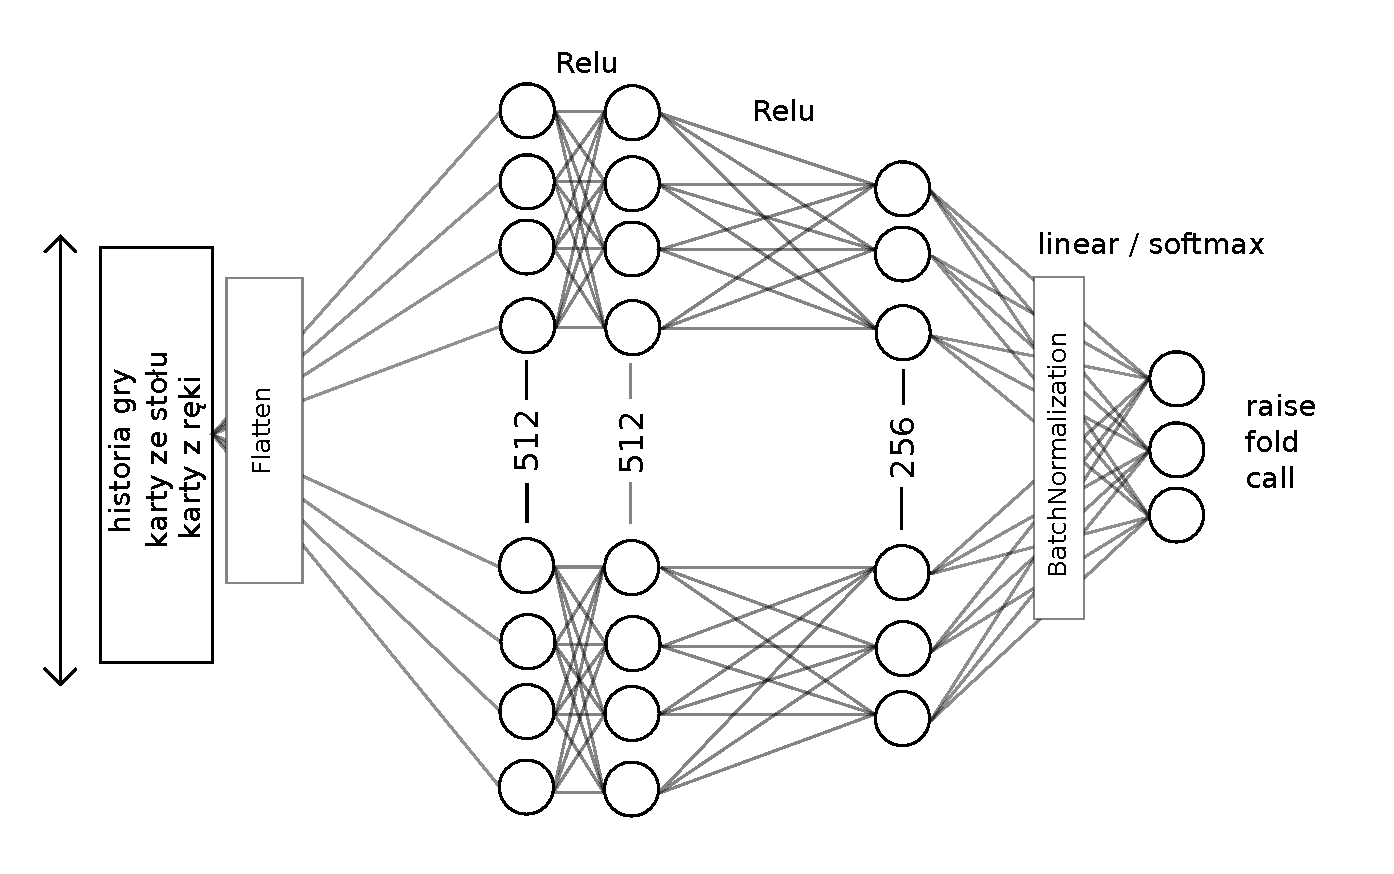
\includegraphics[width=1\textwidth]{./img/nn.pdf}
  \caption{Architektura sieci neuronowych wykorzystana w programie.}
\end{figure}


W trakcie trenowania sieci korzystają z funkcji optymalizującej Adam.
Prędkość uczenia jest równa 0,0001, co spowoduje powolne uczenie, ale zminimalizuje szanse na
ominięcie minimum globalnego. 

Jak wynika z dokumentu prezentującego algorytm Deep CFR, uzyskuje on lepsze wyniki, jeśli sieci
neuronowe są uczone za każdym razem od początku przy losowo ustawionych zerach w wagach \cite{DCFR}. 
W tym celu ustawiono w każdej warstwie funkcję, która tworzy losowo wartości w przedziałach od
-0,005 do 0,005.

Ostatnim elementem sieci jest funkcja licząca błąd predykcji w trakcie uczenia. Jak wynika z 
opisu algorytmu Deep CFR, wymaga on zmodyfikowanej wersji MSE (\emph{Mean Square Error}).
Zostało to wykonane przy pomocy 
funkcji matematycznych na tensorach, jakie udostępnia \emp{Tensorflow} \cite{tensorflow}.


\subsection{Budowa zbiorów danych}

Jak wynika z algorytmu Deep CFR, w programie muszą być zawarte trzy bufory.
Maksymalna pojemność kontenerów $B_{1}$ i $B_{2}$ jest równa 100 000 próbek.
Bufor $B_{s}$ może posiadać ich 200 000. Każdy z dodatnych elementów do bufora składa się z
trzech połączonych wektorów o rozmiarach 52.

Zaimplementowano klasę $\emph{Memory}$ zarządzającą tymi buforami, które zachowują się jak 
kolejki, w przypadku przepełnienia jest usuwany najstarszy wpis.

Mając uzupełnione dane w tablicach, program rozpoczyna przygotowanie zbiorów danych do uczenia
wybranych
sieci neuronowych. Każdy z buforów zostaje losowo przetasowany i podzielony na dwa podzbiory.
Pierwszy z nich to zbiór uczący. Wykorzystuje się go do poprawiania wag modelu sekwencyjnie.
Drugim zbiorem
są dane walidacyjne. Dokonanie takiego podziału było wymagane, aby przeciwdziałać stanowi
przetrenowania modelu. Zbiór walidacyjny jest nadzorowany i na jego podstawie można określić 
moment od, którego model przestaje dobrze działać. Schemat tego
podziału przedstawiono na rys. 3.2.

\begin{figure}[!ht]
  \centering
  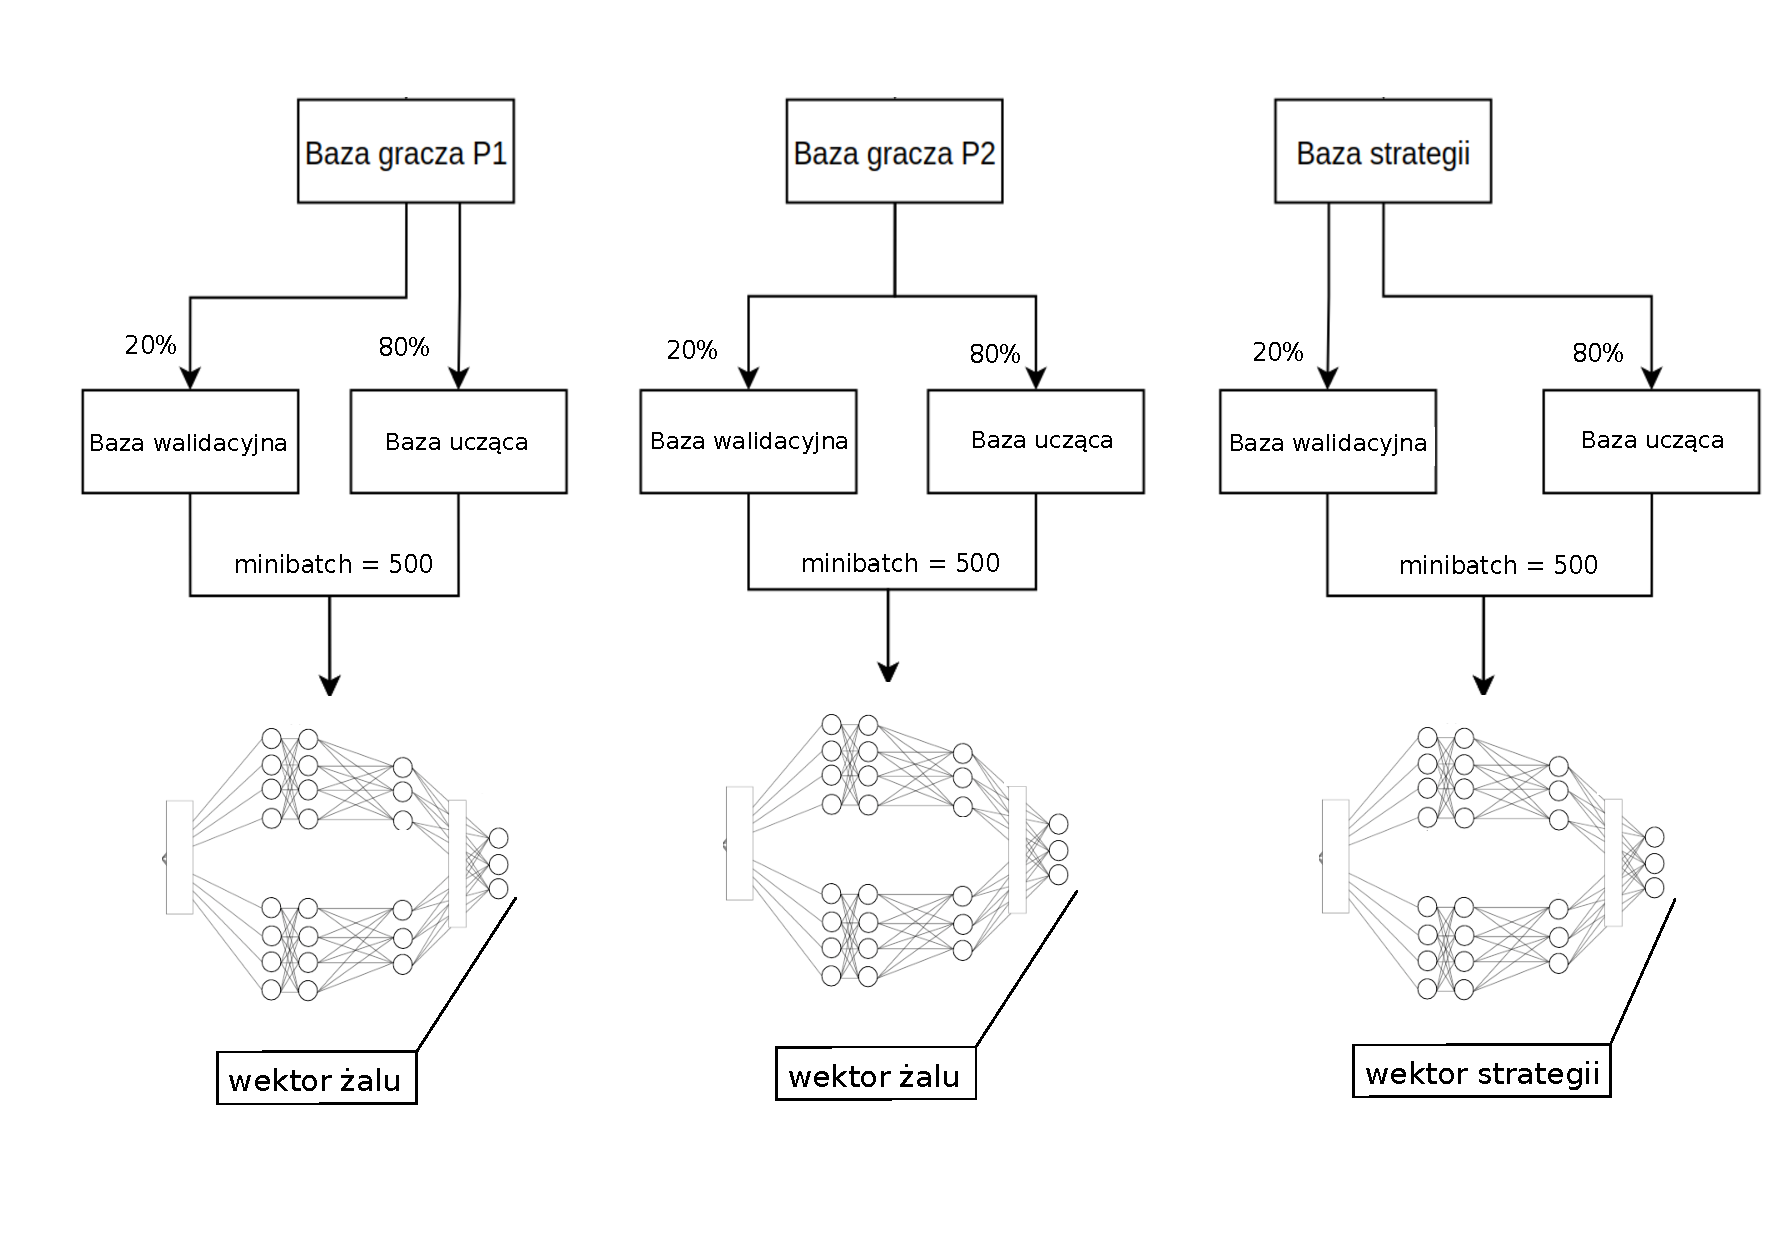
\includegraphics[width=1\textwidth]{./img/bzd.pdf}
  \caption{Podział danych.}
\end{figure}

\vspace{4cm}
W trakcie nauki sieć neuronowa aktualizuje swoje wagi w każdym kroku przez użycie elementu o nazwie
\emph{minibatch} będący parametrem określającym
mały podzbiór bazy użyty do trenowania sieci w pojedynczym kroku. Jego liczebność jest równa 500
próbek.

\subsection{Proces uczenia}

Algorytm Deep CFR do eksploracji wykorzystuje metodę MCCFR ES, która eksploruje w jednej iteracji
250 razy drzewo dezyzyjne gromadząc przy tym próbki w buforach.
Po zakończeniu 
wszystkich powtórzeń zachodzi etap uczenia sieci neuronowych $\theta_{1}$, $\theta_{2}$
wykonując maksymalnie 16 000 aktualizacji wag.
Taki schemat działania jest wykonywany dla obu graczy i powtarza się 50 razy. Końcowym
zadaniem jest wytrenowanie sieci neuronowej $\theta_{s}$.  
Wszystkie te elementy zostały połączone przez klasę $\emph{Player}$ posiadającą obiekty
$\emph{Memory}$
oraz $\emph{Network}$, rys. 3.4. 

Dodatkowo w celu poprawienia wyników uczenia użyto funkcji \emp{EarlyStopping} \cite{tensorflow}.
Zatrzymuje ona iteracje modelu w przypadku kiedy błąd predykcji na zbiorze
walidacyjnym wzrośnie odpowiednio wysoko. Jest to sprawdzane na podstawie argumentu \emph{patience},
który określa próg, po którym nauka się kończy. Taka procedura została zastosowana, aby
zminimalizować szanse na przetrenowanie modeli, a wraz z tym ich gorszą jakość \cite{early}.
Rys. 3.3 prezentuje przykładowy punkt zakończenia nauki modelu.

\begin{figure}[!ht]
  \centering
  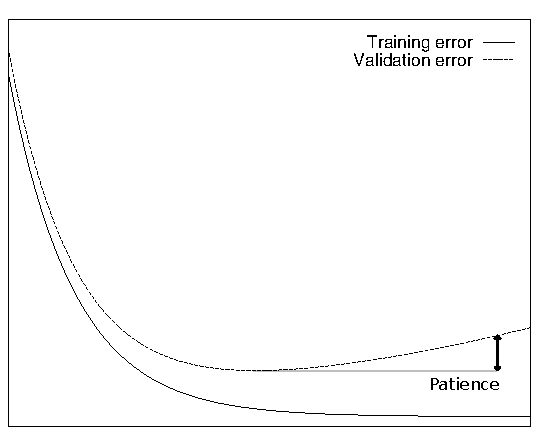
\includegraphics[width=0.7\textwidth]{./img/early.pdf}
  \caption{Przykładowy punkt zatrzymania się uczenia po zastosowaniu \emph{EarlyStopping} \cite{early}.}
\end{figure}

\section{Implementacja środowiska}

Do symulacji gry HULH z którym model będzie się komunikował, użyto blblioteki PyPokerEngine.
Klasa 
\emph{HULH\_Emulator} 
zaimplementowana w programie pozwala na utworzenie obiektu
zarządzającego grą HULH. Przy tworzeniu obiektu zostają zdefiniowane 
nazwy graczy P1 i P2, które w dalszej części będą używane do śledzenia histori gry. 
W tabeli nr 3.3 wylistowano parametry ustawione w programie, związane z zasadami grą.


\begin{table}[h!]
\centering
\caption{Parametry gry HULH.}
\begin{tabular}{|c|c| }
   \hline
   parametr & wartość \\
    \hline
   ante & 0  \\ 
   \hline
   mała w ciemno & 5  \\  
   \hline
   duża w ciemno & 10 \\
   \hline
   liczba rund po których resetuje się środowisko & 1  \\
   \hline
   udział każdego z graczy (stock) & 80  \\
   \hline
   liczba graczy & 2 \\
   \hline
\end{tabular}
\end{table}

Zaimplementowane środowisko opiera się na PyPokerEngine, co oznacza, że każda akcja zwraca dwa
elementy, obiekt określający stan gry oraz historię gry w formie json. Obie wartości są używane do
śledzenia stanu środowiska w drzewie decyzyjnym. Informacje jak karty na stole, historia gry lub 
wygrana gracza jest zarządzane przez użytą bibliotekę. Napisane funkcje w programie pełnia tylko 
zadanie interfejsu dla drzewa.


\section{Implementacja Deep CFR}

Klasa \emph{DCFR} zawiera implementację algorytmu Deep CFR. 
Przy tworzeniu obiektu powstają w
konstruktorze trzy elementy gracz, oponent oraz strategia $\sigma$ z klasy \emph{Brain}.
Do tego ustawiane jest środowisko \emph{HULH\_Emulator} przez referencje.

Cały proces powstawania modelu rozpoczyna się od funkcji \emph{iterate}, która wykonuje trzy pętle
\emph{for},
dla iteracji algorytmu i powtórzeń eksploracji drzewa dla każdego z graczy. W pierwszej z nich 
środowisko tworzy nową grę, w ostatniej pętli jest wykonywana funkcja \emph{\_\_traverse},
działająca wedłóg metody MCCFR ES. Dostaje ona argumenty \emph{state} czyli obiekt określający
stan gry, \emph{events} - dotychczasową historię oraz \emph{timestep}.
Ostatni argument \emph{verbose} jest opcialny i służy tylko do wizualizacji powstałego drzewa
decyzyjnego. Funckja działa po przez rekurencję.
Po zakończeniu działania MCCFR ES, rozpoczyna się uczenie sieci neuronowej $\theta_{p}$. I
powtażanie powyrzszego procesu. 
Ostatnim etapem jest trenowanie sieci $\theta_{s}$ oraz zapisanie jej do pliku.
Tab. 3.4 prezentuje podstawowe parametry zaimplementowanego algorytmu.


\begin{table}[h!]
\centering
\caption{Parametry algorytmu Deep CFR.}
\begin{tabular}{|c|c| }
   \hline
   parametr & wartość \\
    \hline
   liczba powtórzeń eksploracj drzewa & 250  \\ 
   \hline
   liczba iteracji algorytmu & 50  \\  
   \hline
   co ile iteracji wytrenować i zapisać model & 10 \\
   \hline
\end{tabular}
\end{table}





\begin{figure}[!ht]
  \centering
  \hspace*{-1cm}   
  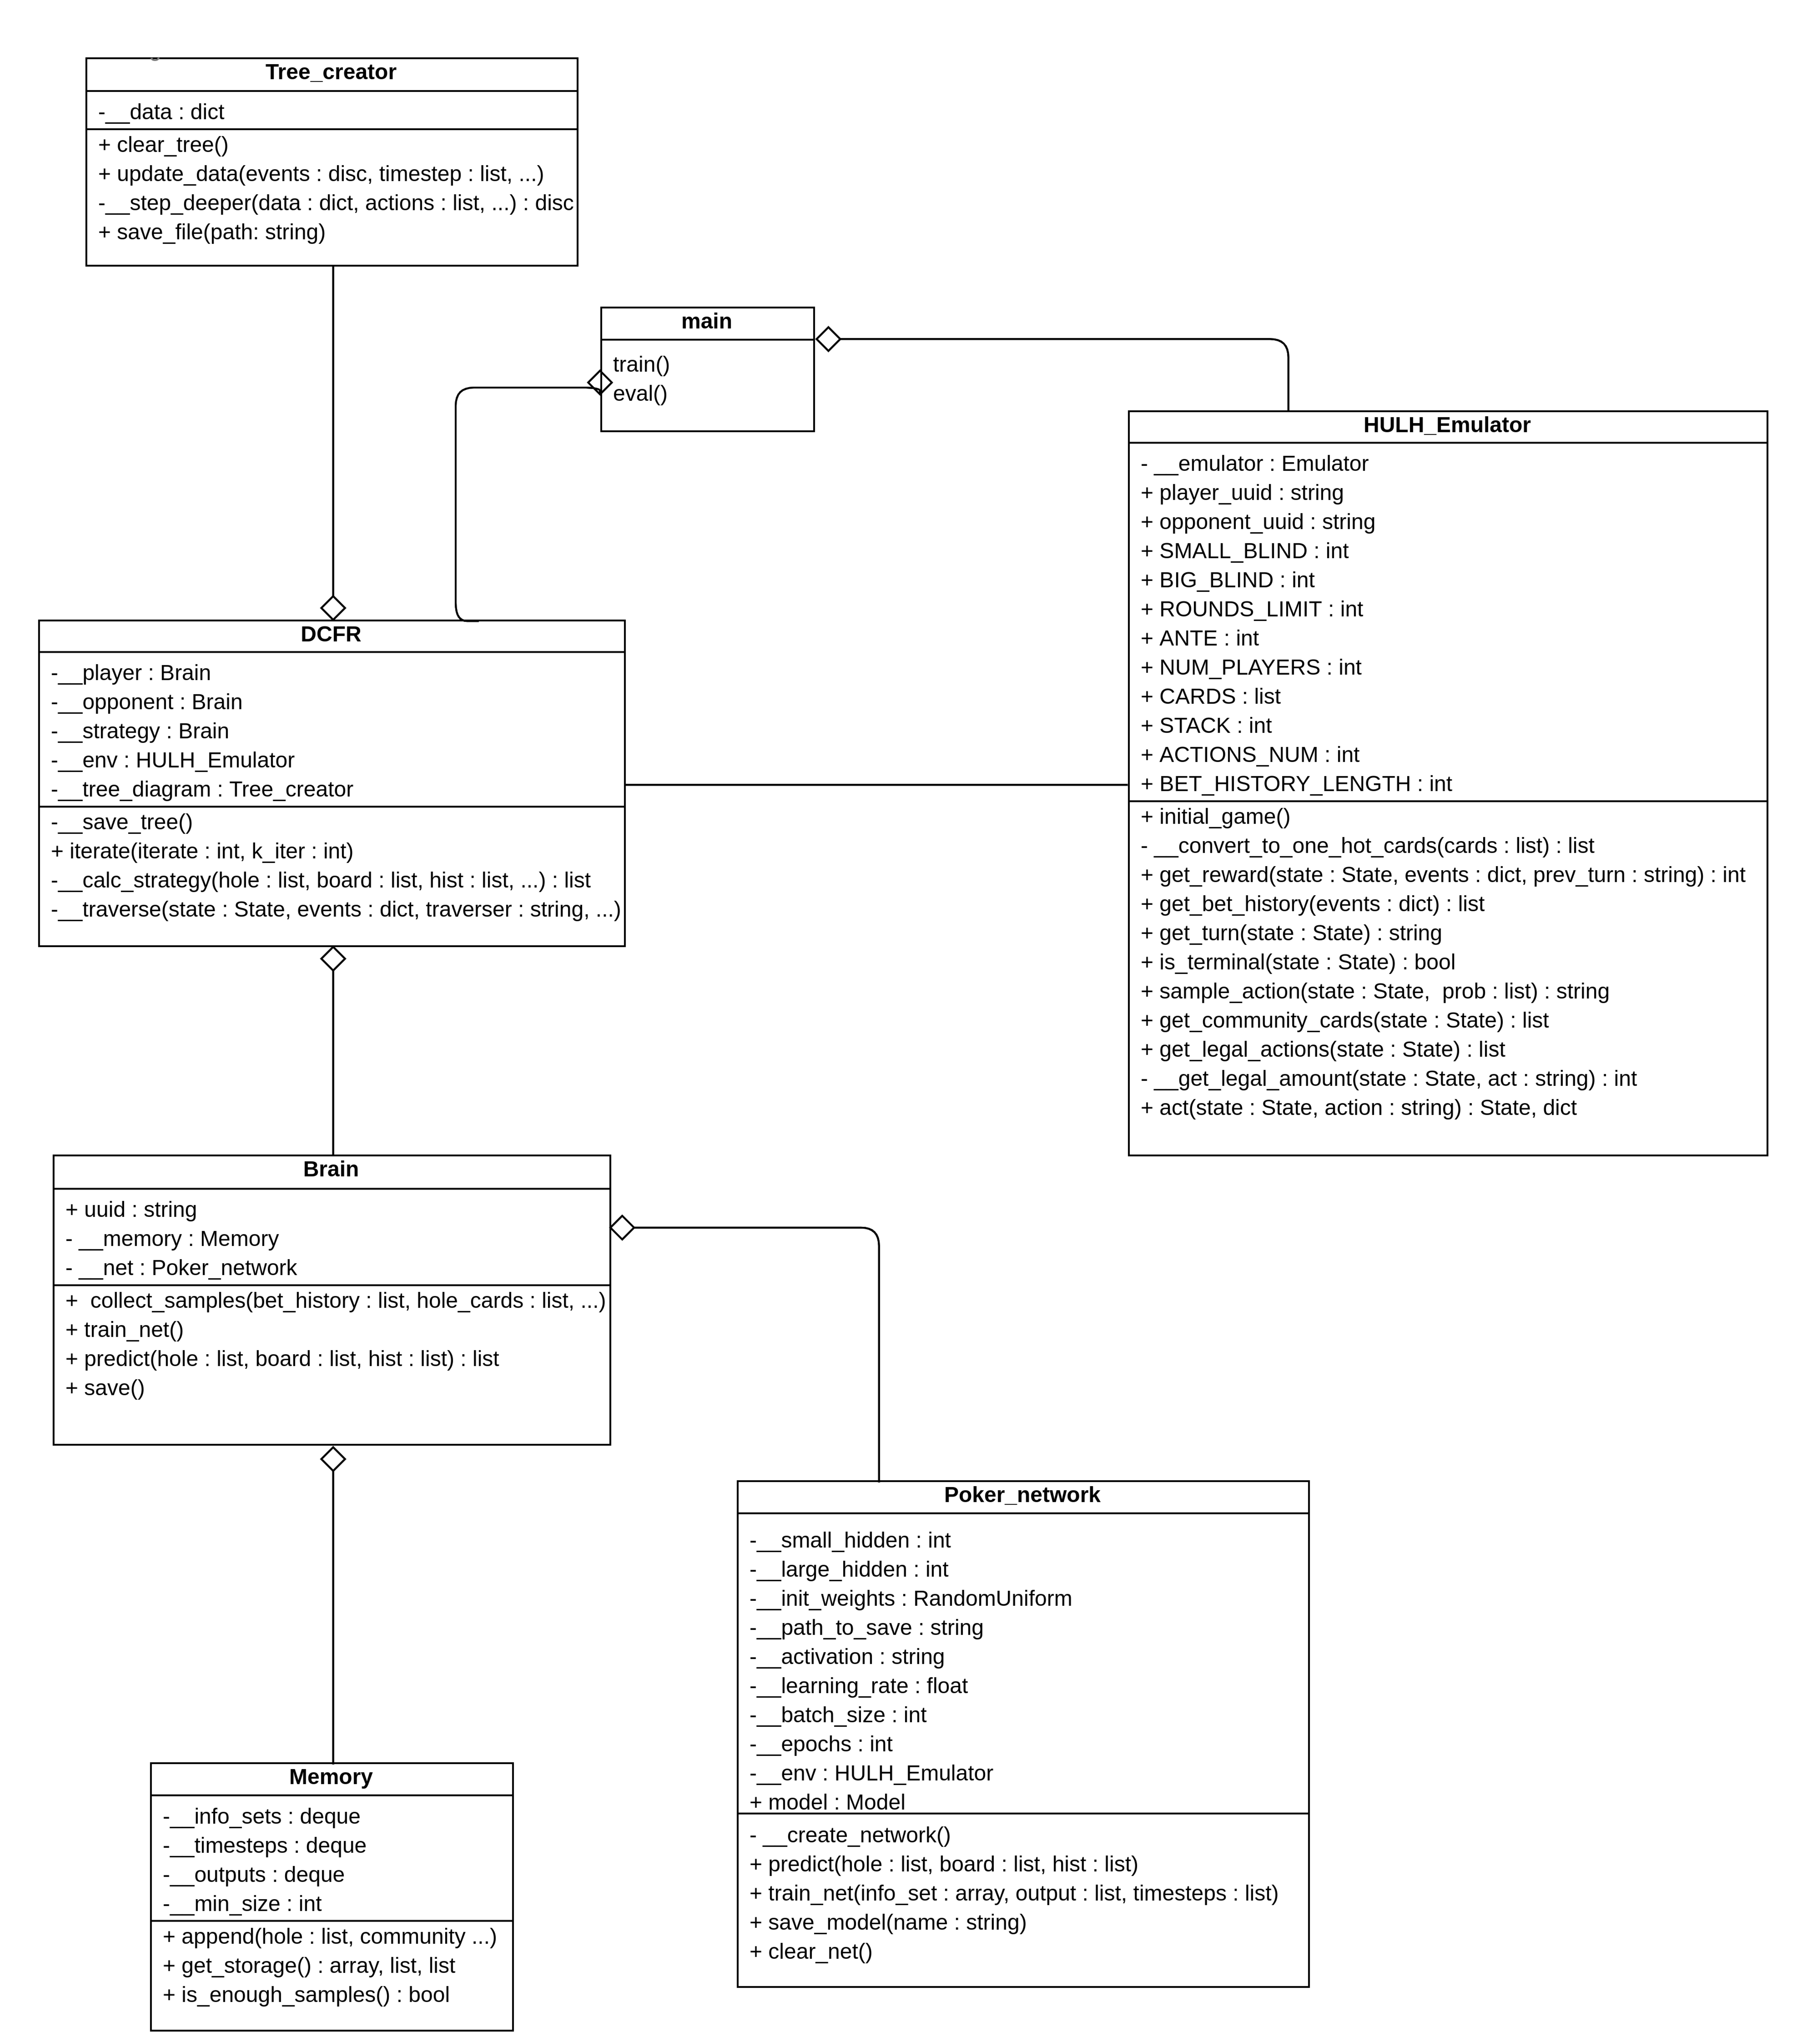
\includegraphics[width=1.1\textwidth]{./img/uml.pdf}
  \caption{Diagram UML projektu.}
\end{figure}

\section{Podsumowanie}

\chapter{Wyniki}

Rozdział przedstawia różnice między utworzonymi modelami z algorytmu Deep CFR. Zostały tutaj
zaprezentowane wykresy jakości uczenia oraz wyniki rozegranych gier między nimi wraz z zwycięscą.


\section{Proces uczenia modelów rozpoznawania}

Algorytm Deep CFR pracując przez trzy dni zdołał utworzyć pięć modeli, gdzie każda nauka była
śledzona przez bibliotekę \emph{TensorBoard}. Uzyskane dane następnei zostały zaimportowane do
Excela w celu utworzenia czytelnych wykresów ilustrujących zalezność błędu predykcji od liczby
iteracji.

Pierwszy utworzony model powstał po 10 powtórzeniach algorytmu. Jak można zobaczyć na rys. 4.1
wartość błędu
zbiegła się bardzo szybko do wartości bliskiej 0 dla zbioru uczącego i walidacyjnego. Wynika to z 
małej liczby zebranych próbek w buforze $B_{s}$ o małej różnorodności. Po mimo tak dobrych efektów
można zauwazyć na rys. 4.2, że model nr 1 nie wygrał tylko z modelem nr 3 z nie wielką przewagą.

\begin{figure}[!ht]
  \centering
  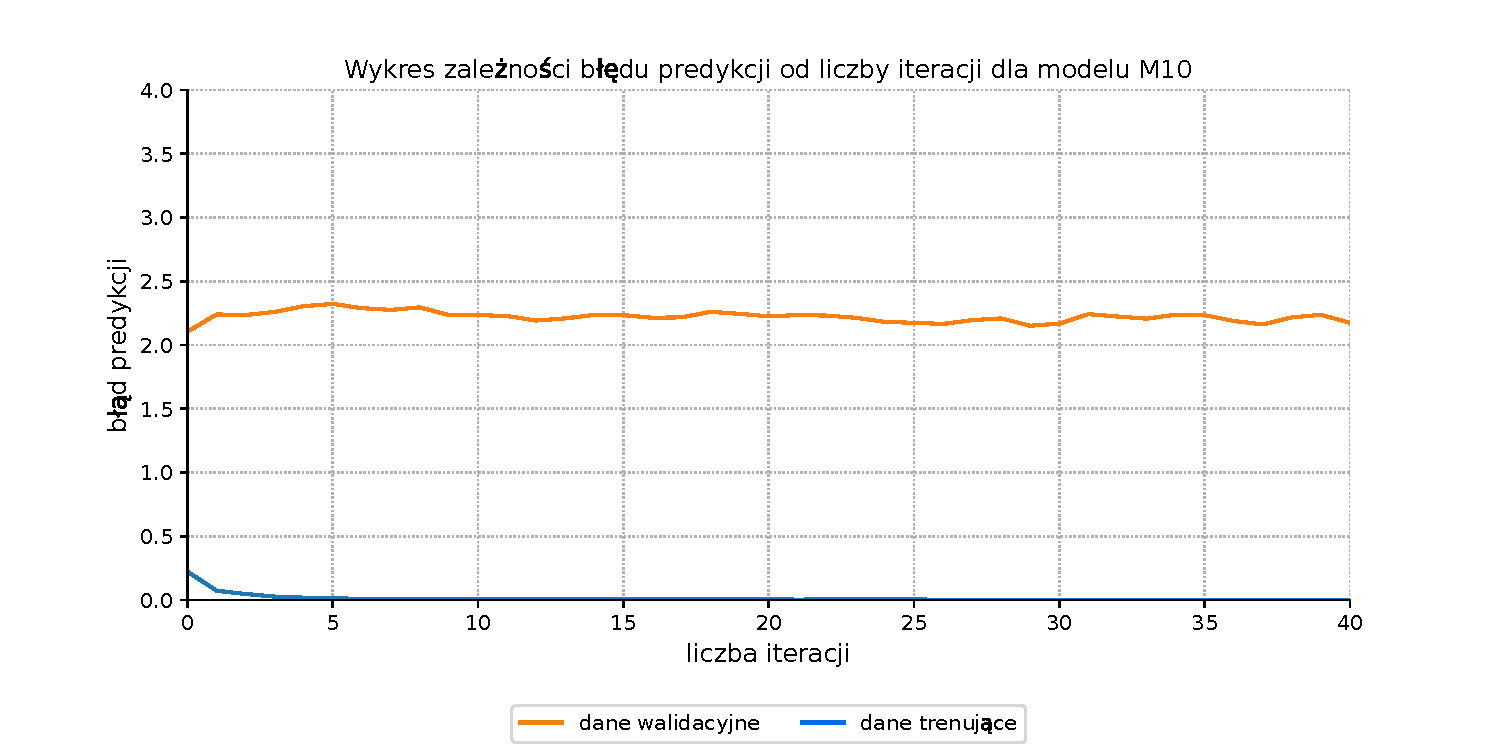
\includegraphics[width=1\textwidth]{./img/model1.pdf}
\caption{Wyniki uczenia modelu nr 1.}
\end{figure}

\begin{figure}[!ht]
  \centering
  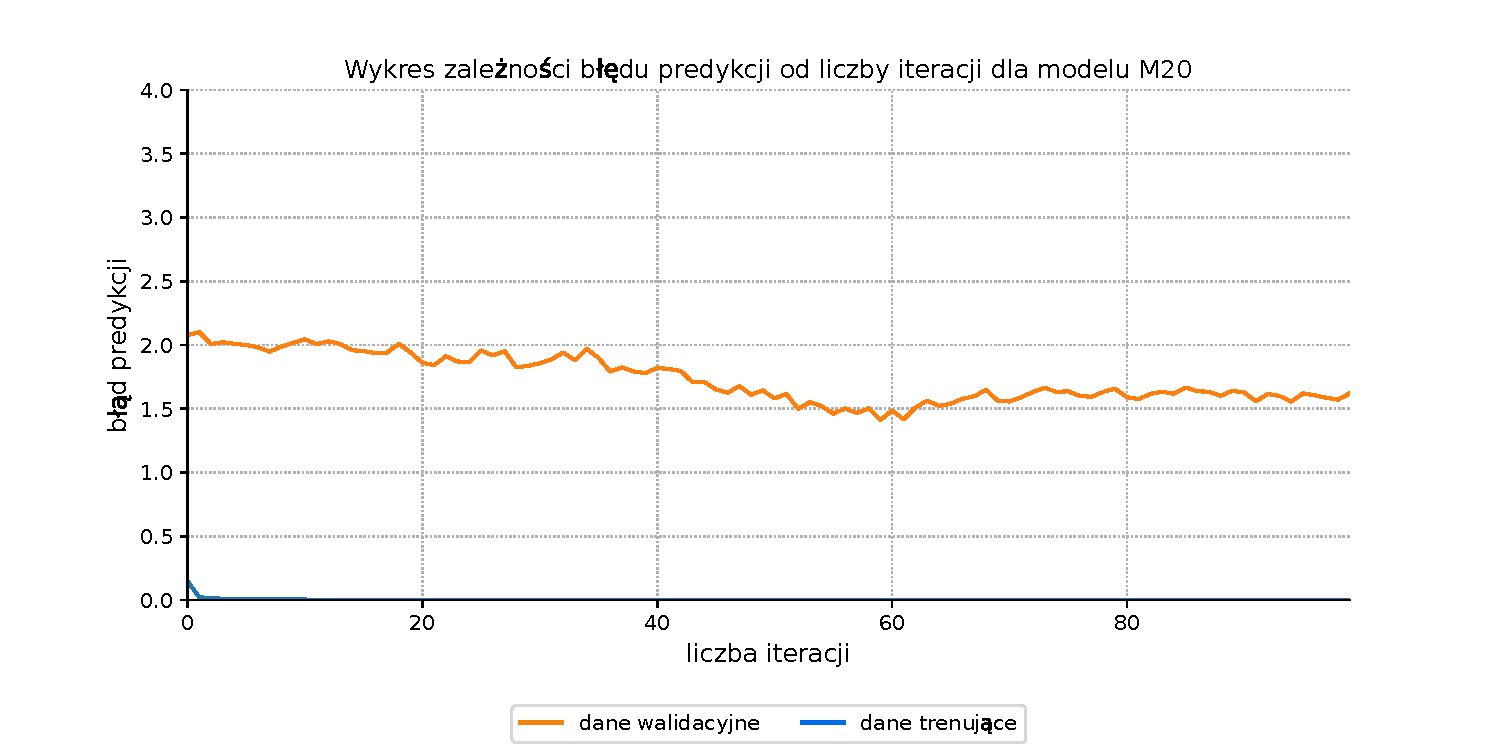
\includegraphics[width=1\textwidth]{./img/model2.pdf}
\end{figure}

\begin{figure}[!ht]
  \centering
  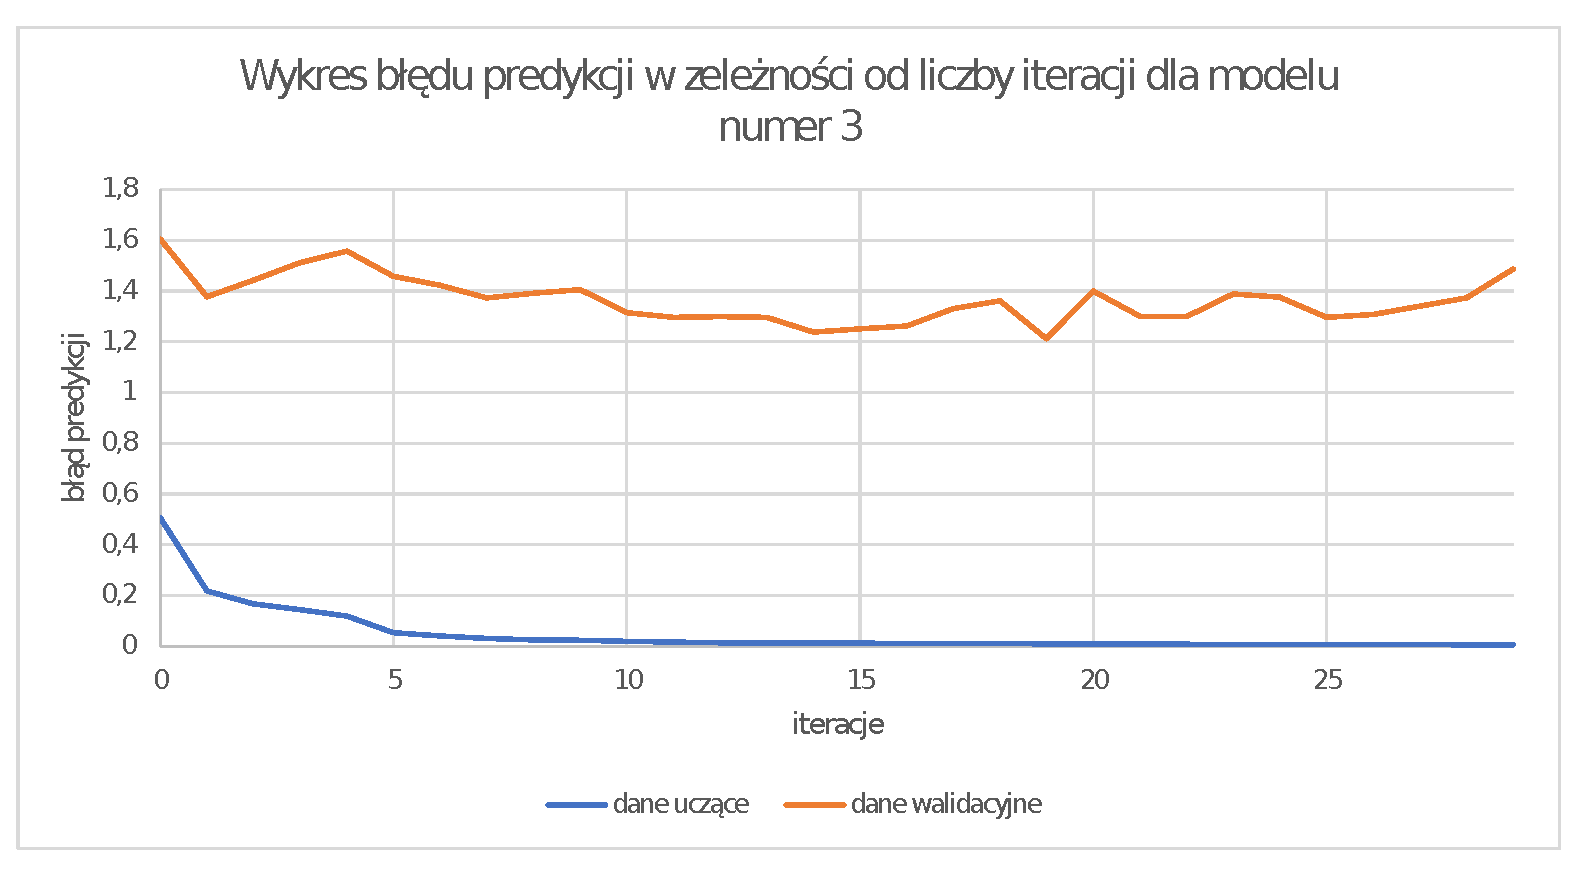
\includegraphics[width=1\textwidth]{./img/model3.pdf}
\end{figure}

\begin{figure}[!ht]
  \centering
  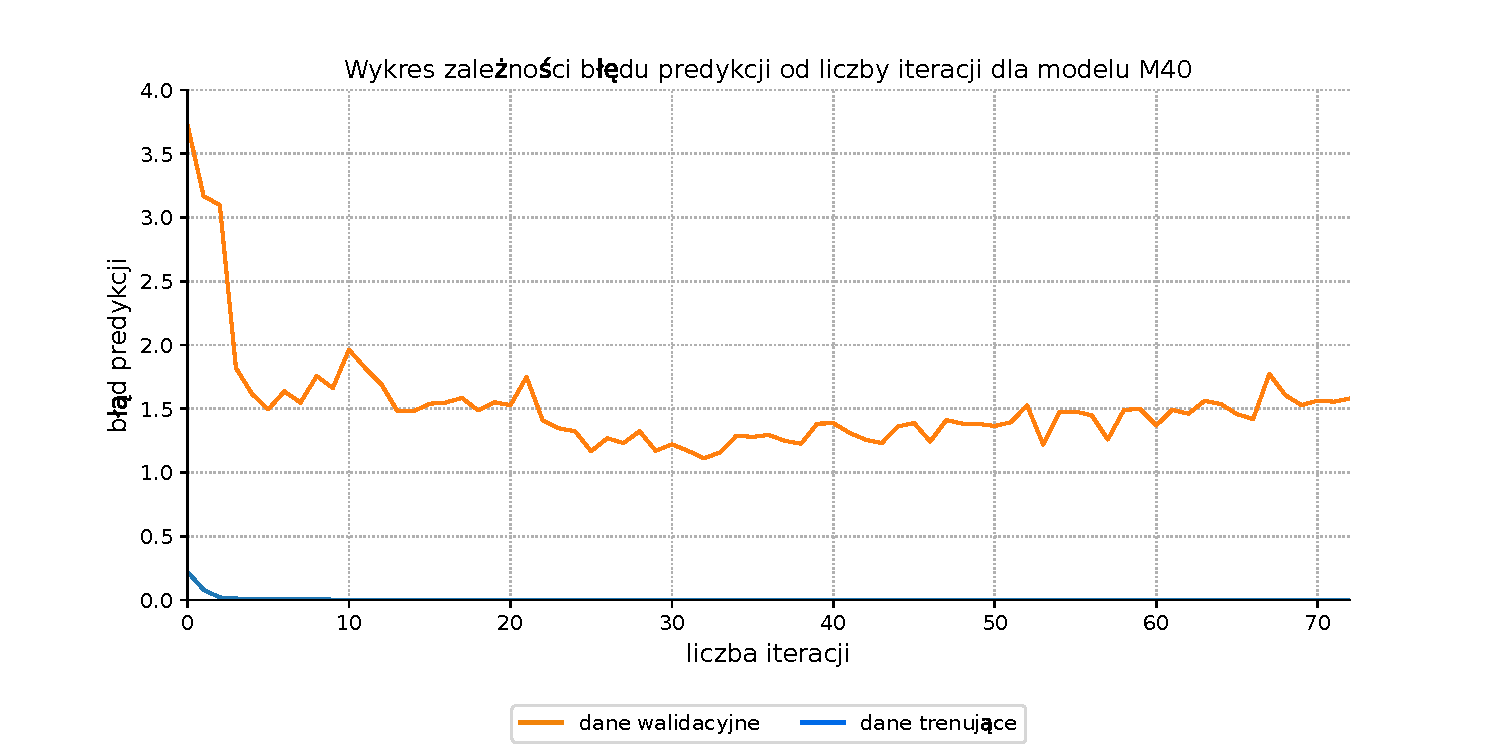
\includegraphics[width=1\textwidth]{./img/model4.pdf}
\end{figure}
\begin{figure}[!ht]
  \centering
  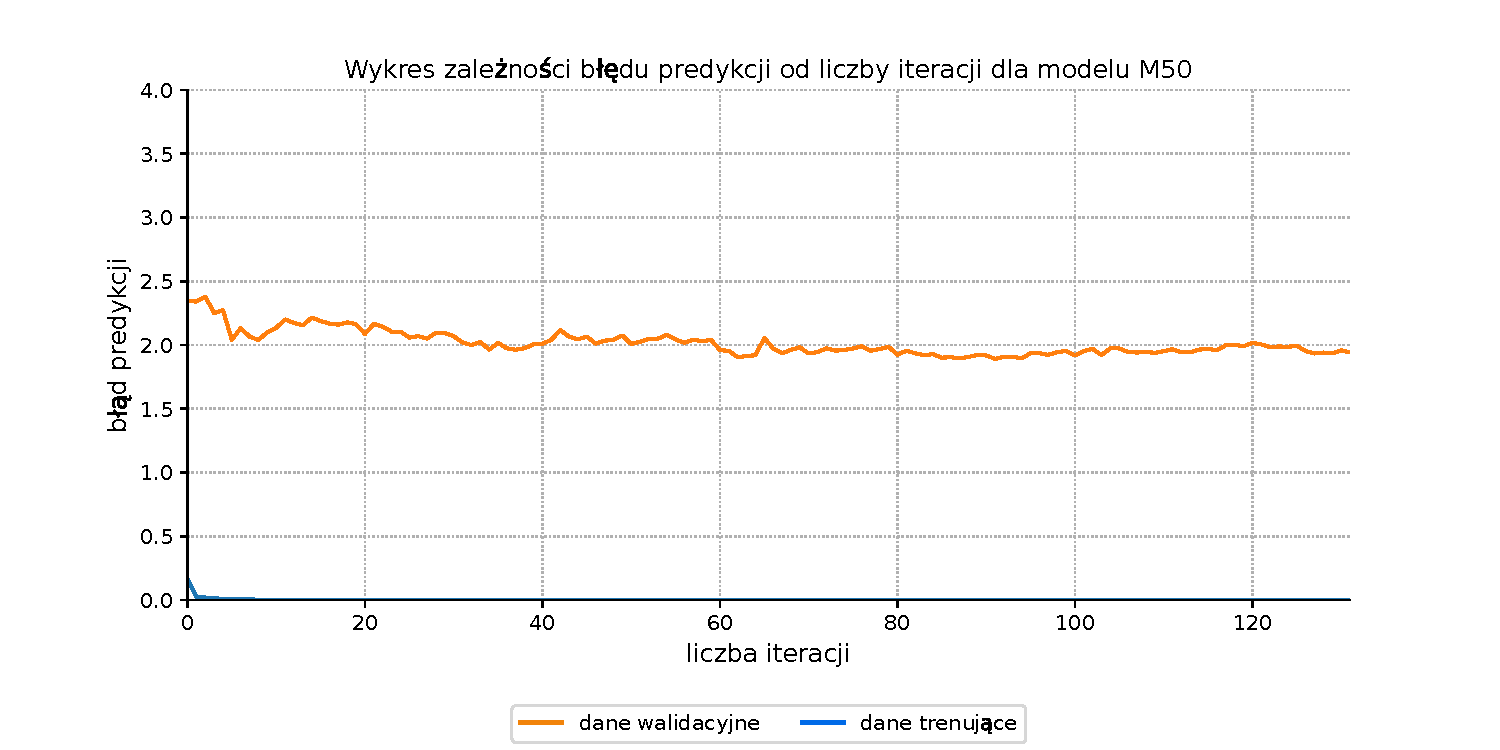
\includegraphics[width=1\textwidth]{./img/model5.pdf}
\end{figure}
\section{Wyniki rozgrywek modeli}

\begin{figure}[!ht]
  \centering
  \hspace*{-1cm}   
  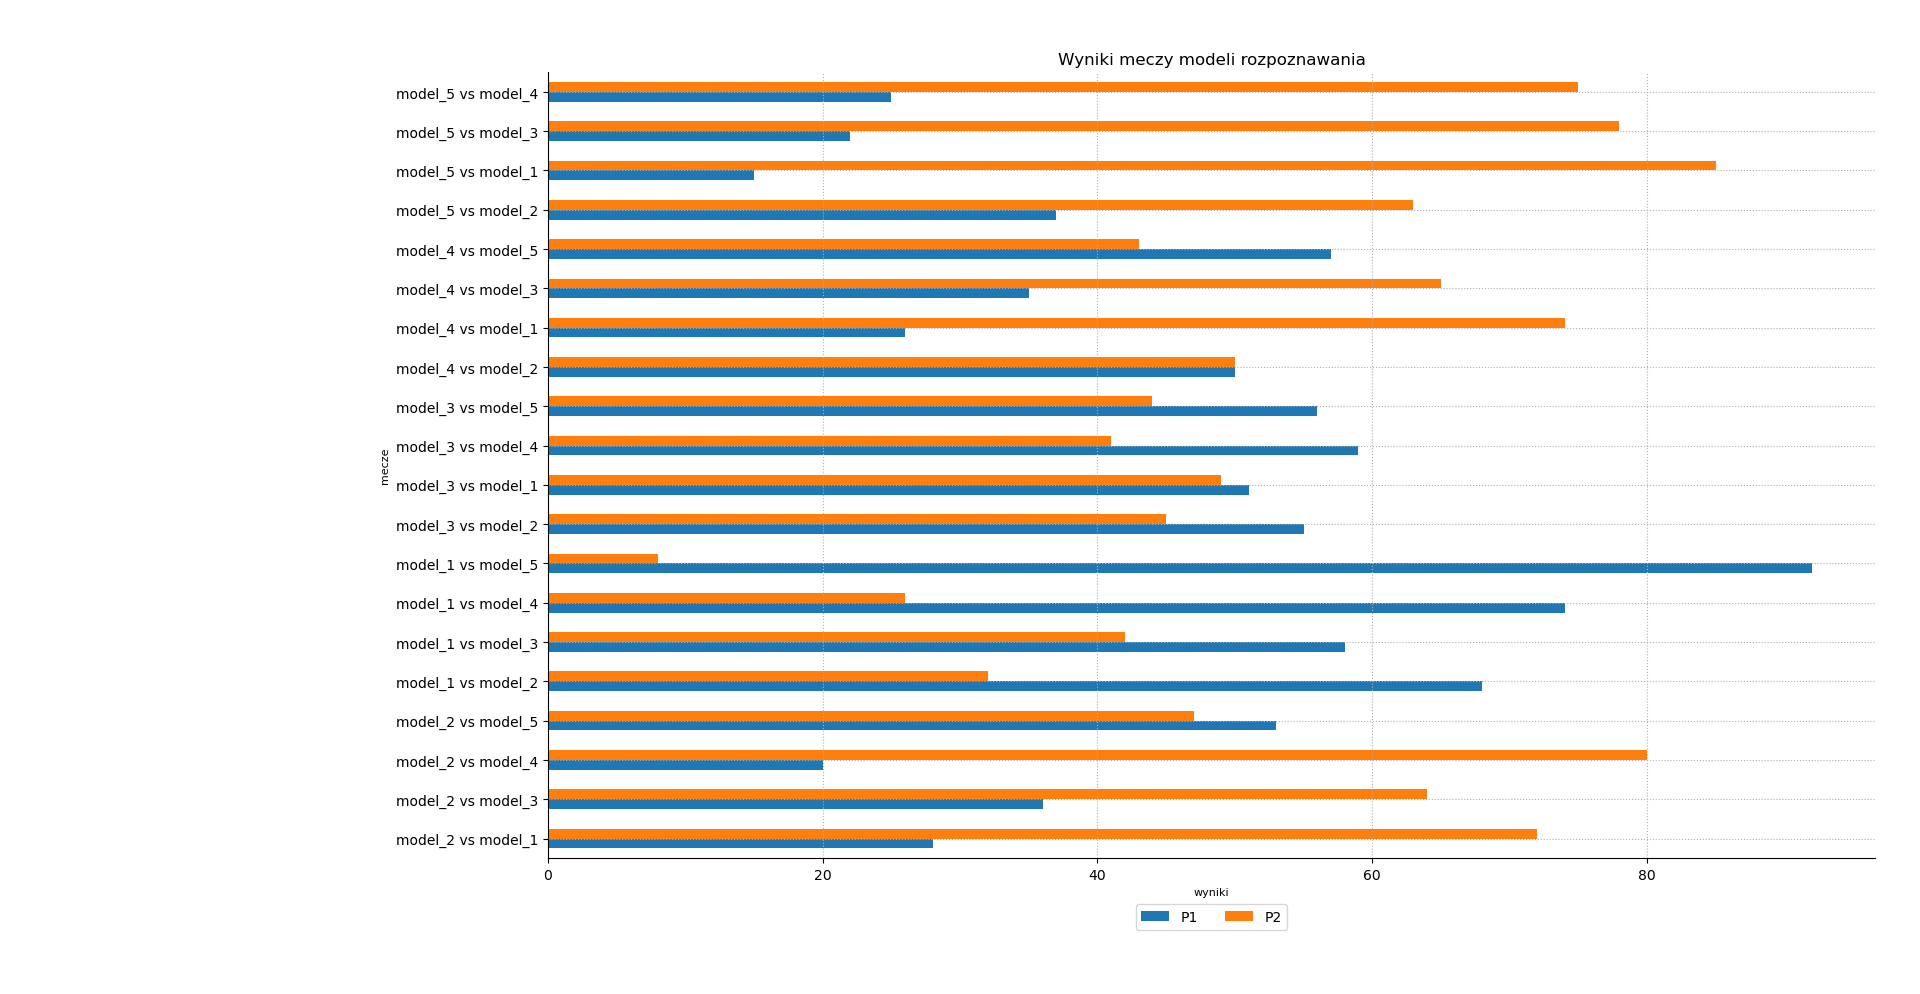
\includegraphics[width=1.1\textwidth]{./img/mecze.png}
  \caption{Diagram UML projektu.}
\end{figure}

\begin{thebibliography}{100}
   \bibitem{hist AI} Haenlein, Michael, and Andreas Kaplan. "A brief history of artificialintelligence: On the past, present, and future of artificial intelligence." California management review 61.4 (2019): 5-14.
   \bibitem{Go} Gibney, Elizabeth. "Google AI algorithm masters ancient game of Go." Nature News 529.7587 (2016): 445.
   \bibitem{Dota2} Berner, Christopher, et al. "Dota 2 with large scale deep reinforcement learning." arXiv preprint arXiv:1912.06680 (2019).
   \bibitem{iig} Brown, Noam, et al. "Combining deep reinforcement learning and search for imperfect-information games." arXiv preprint arXiv:2007.13544 (2020).

   \bibitem{DCFR} Brown, Noam, et al. "Deep counterfactual regret minimization." International conference on machine learning. PMLR, 2019. 
   \bibitem{XFP} Heinrich, Johannes, Marc Lanctot, and David Silver. "Fictitious self-play in extensive-form games." International conference on machine learning. PMLR, 2015.
   \bibitem{CFR} Zinkevich, Martin, et al. "Regret minimization in games with incomplete information." Advances in neural information processing systems 20 (2007): 1729-1736.
   \bibitem{NFSP} Heinrich, Johannes, and David Silver. "Deep reinforcement learning from self-play in imperfect-information games." arXiv preprint arXiv:1603.01121 (2016).

   \bibitem{poker} Teófilo, Luís Filipe Guimarães. "Building a poker playing agent based on game logs using supervised learning." (2010).
   \bibitem {theory poker} Bouju, Gaëlle, et al. "Texas hold'em poker: a qualitative analysis of gamblers' perceptions." Journal of Gambling Issues 28 (2013): 1-28.
   \bibitem{class} Félix, Dinis Alexandre Marialva. "Artificial intelligence techniques in games with incomplete information: opponent modelling in Texas Hold'em." (2008).
   \bibitem{mdp} Xiang, Xuanchen, and Simon Foo. "Recent Advances in Deep Reinforcement Learning Applications for Solving Partially Observable Markov Decision Processes (POMDP) Problems: Part 1—Fundamentals and Applications in Games, Robotics and Natural Language Processing." Machine Learning and Knowledge Extraction 3.3 (2021): 554-581.

   \bibitem{rn}  Nogal-Meger, P. (2012). Dylemat więźnia jako przykład wykorzystania teorii gier. Prace i Materiały Wydziału Zarządzania Uniwersytetu Gdańskiego, 10(4, cz. 2), 87–95.
   \bibitem{gt} Myerson, Roger B. Game theory. Harvard university press, 2013.
   \bibitem{cepheus} Bowling, Michael, et al. "Heads-up limit hold'em poker is solved." Communications of the ACM 60.11 (2017): 81-88.
   \bibitem{ds} Moravčík, Matej, et al. "Deepstack: Expert-level artificial intelligence in heads-up no-limit poker." Science 356.6337 (2017): 508-513. 
   \bibitem{ss} Davis, Trevor, Neil Burch, and Michael Bowling. "Using response functions to measure strategy strength." Twenty-Eighth AAAI Conference on Artificial Intelligence. 2014. 
   \bibitem{mccfr} Lanctot, Marc, et al. "Monte Carlo sampling for regret minimization in extensive games." Advances in neural information processing systems 22 (2009): 1078-1086.
   \bibitem{early} Prechelt, Lutz. "Early stopping-but when?." Neural Networks: Tricks of the trade. Springer, Berlin, Heidelberg, 1998. 55-69.

   \bibitem{numpy} Harris, C.R., Millman, K.J., van der Walt, S.J. et al. Array programming with NumPy. Nature 585, 357–362 (2020)
   \bibitem{tensorflow} Martín Abadi, Ashish Agarwal, Paul Barham, Eugene Brevdo,
Zhifeng Chen, Craig Citro, Greg S. Corrado, Andy Davis,
Jeffrey Dean, Matthieu Devin, Sanjay Ghemawat, Ian Goodfellow,
Andrew Harp, Geoffrey Irving, Michael Isard, Rafal Jozefowicz, Yangqing Jia,
Lukasz Kaiser, Manjunath Kudlur, Josh Levenberg, Dan Mané, Mike Schuster,
Rajat Monga, Sherry Moore, Derek Murray, Chris Olah, Jonathon Shlens,
Benoit Steiner, Ilya Sutskever, Kunal Talwar, Paul Tucker,
Vincent Vanhoucke, Vijay Vasudevan, Fernanda Viégas,
Oriol Vinyals, Pete Warden, Martin Wattenberg, Martin Wicke,
Yuan Yu, and Xiaoqiang Zheng.
TensorFlow: Large-scale machine learning on heterogeneous systems,
2015. Software available from tensorflow.org.
\end{thebibliography}



\end{document}

